%
% Chapter 7
%

\chapter{Background Estimation}
\label{bkg_est}

\section{Introduction}
The dominant background contribution comes from the \Ztt process, in which the muon or electron arises from a tau decay. The other dominant background contribution comes from \wjets and QCD multijets processes, where one or more of the jets are misidentified as leptons. In the leptonic channels, the \ttbar process also has a dominant background contribution.

Other background contributions come from the processes in which a lepton pair is produced from the weak decays of quarks and vector bosons. These processes include Higgs boson production (\Htt, \PW{}\PW), \PW{}\PW, \PW{}\PZ, and \PZ{}\PZ. There are non-negligible contributions from processes like $\PW\Pgg^{(\ast)} +$ jets, single top quark production, and \Zll $(\ell=\Pe,\Pgm)$. Feynman diagrams of background processes to LFV Higgs boson decays are shown in Figure~\ref{fig:feynman_bkg}.

The dominant contributors, \Ztt and misidentified lepton backgrounds are estimated from data using either a fully data-driven or semi data-driven approach. All the other backgrounds are estimated from simulated samples. The background estimates are validated in different orthogonal control regions constructed to have enhanced contributions from the dominant backgrounds.

\begin{figure}[htbp!]
  \centering
  \subfigure[]{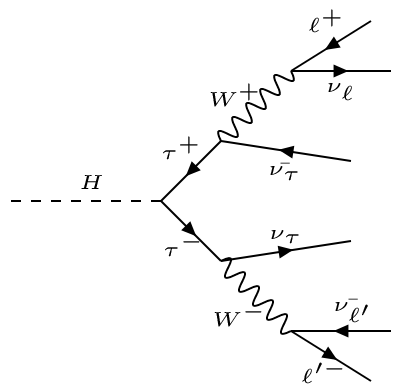
\includegraphics[width=0.3\textwidth]{plots/chapter7/Feynman/Htt.png}}
  \hspace{0.5cm}
  \subfigure[]{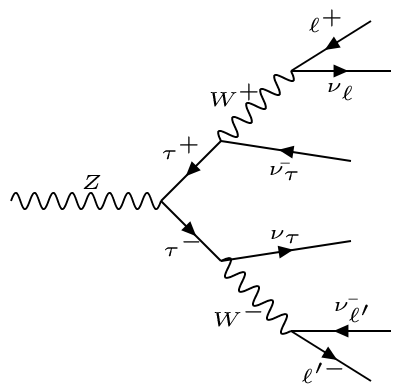
\includegraphics[width=0.3\textwidth]{plots/chapter7/Feynman/Ztt.png}}
  \hspace{0.5cm}
  \subfigure[]{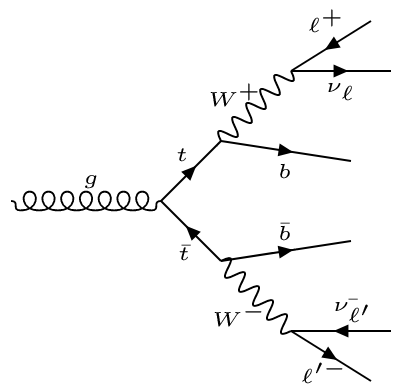
\includegraphics[width=0.3\textwidth]{plots/chapter7/Feynman/ttbar.png}}\\
  \vspace{1cm}
  \subfigure[]{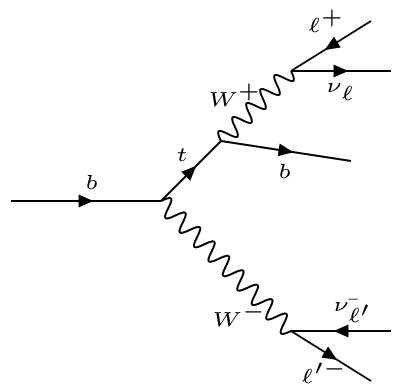
\includegraphics[width=0.3\textwidth]{plots/chapter7/Feynman/tW.png}}
  \hspace{0.5cm}
  \subfigure[]{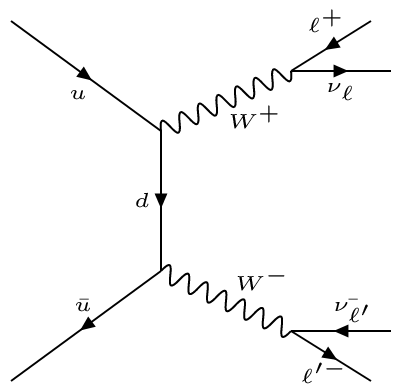
\includegraphics[width=0.3\textwidth]{plots/chapter7/Feynman/WW.png}}
  \hspace{0.5cm}
  \subfigure[]{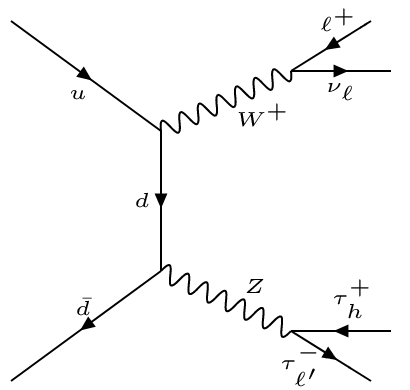
\includegraphics[width=0.3\textwidth]{plots/chapter7/Feynman/WZ.png}}\\
  \vspace{1cm}
  \subfigure[]{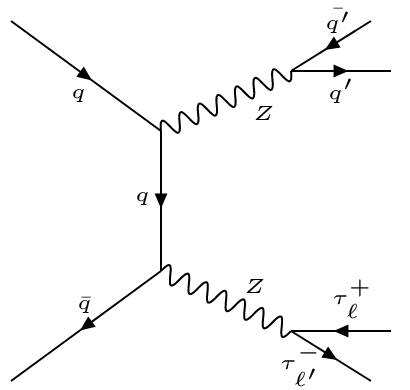
\includegraphics[width=0.3\textwidth]{plots/chapter7/Feynman/ZZ.png}}
  \hspace{0.5cm}
  \subfigure[]{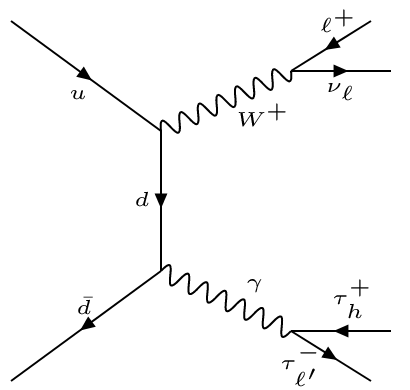
\includegraphics[width=0.3\textwidth]{plots/chapter7/Feynman/WG.png}}\\
  \caption{Feynman diagrams of background processes to LFV Higgs boson decays: (a) \Htt, (b) \Ztt, (c) \ttbar, (d) Single Top, (e) \PW{}\PW, (f) \PW{}\PZ, (g) \PZ{}\PZ, and (h) $\PW\Pgg^{(\ast)}$.}
  \label{fig:feynman_bkg}
\end{figure}

\section{Embedding technique}
The \Ztt background is estimated from data using the embedding technique~\cite{Sirunyan:2019drn}. The embedding technique allows for an estimation of the genuine \Pgt{}\Pgt SM backgrounds from data that minimizes uncertainties arising from a poor event description, with minimal simulation input. Events with a pair of oppositely charged muons are selected in data so that \Zmm events largely dominate it. These data events are chosen independently of the event selection criteria described in chapter~\ref{event_sel}.

The muons are removed from the selected events and replaced with simulated tau leptons with the same kinematic properties as that of the replaced muon. In that way, a set of hybrid events is obtained that relies on simulation only for the decay of the tau leptons. The description of the underlying event or the production of associated jets is taken entirely from data, and there is no reliance on the simulation. This technique results in a more accurate description of the \ptvecmiss, jet related variables, and an overall reduction in the systematic uncertainties that arise due to the usage of simulated samples.

Embedded samples cover all backgrounds with two real tau leptons decaying semi-hadronically or leptonically. This includes a small fraction of \ttbar, Diboson, and electroweak \PW/\PZ events. The events from the \ttbar, Diboson, and electroweak \PW/\PZ MC samples where both tau candidates match genuine taus at the generator level are removed to avoid any double counting. A schematic for the embedding technique can be seen in Figure~\ref{fig:embedding}.

\begin{figure}[htbp!]
  \centering
  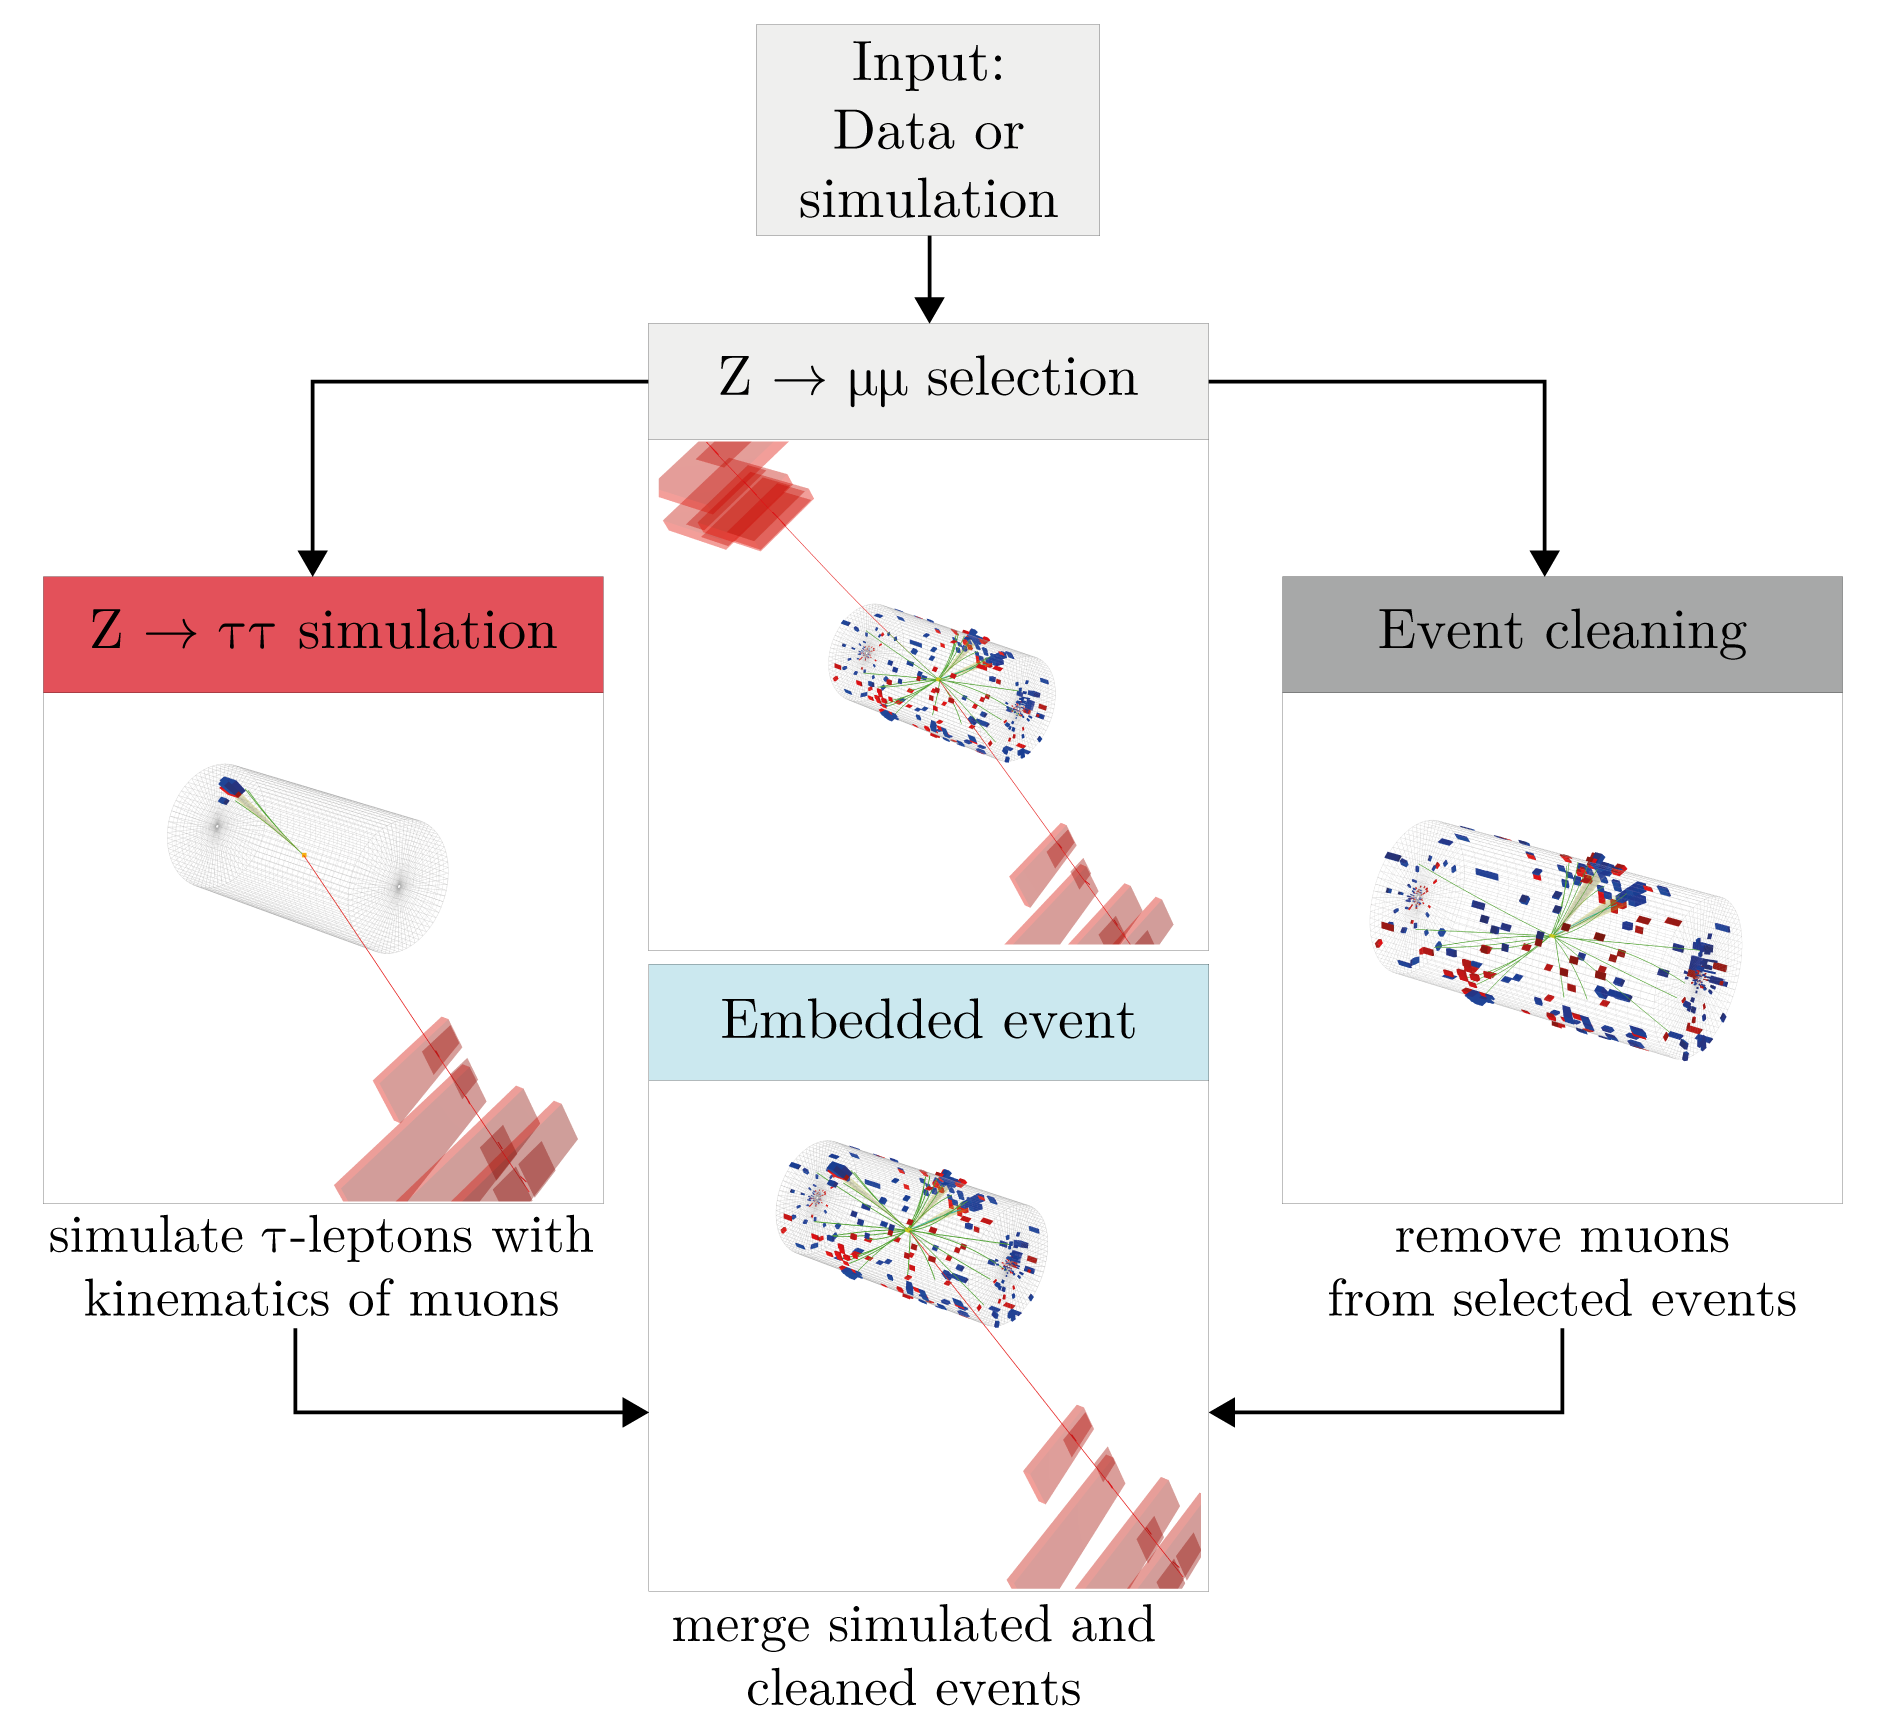
\includegraphics[width=0.8\textwidth]{plots/chapter7/emb.png}
  \caption{Schematic of embedding technique}
  \label{fig:embedding}
\end{figure}

The \Ztt background is validated by looking at the agreement between observed data and estimated background in a region enriched with \Ztt events. In \muhad channel, this region is constructed by requiring, in addition to the preselection, $\mt(\Pgm) < 40 \GeV$, $40 \GeV < \mvis(\Pgm, \Pgt) < 80 \GeV$, and $\pzeta(\Pgm, \Pgt) > -25$. \pzeta is the difference of the projections of $\pt^{\ell}$ plus MET, and the $\pt^{\ell}$ on the axis bisecting the two leptons. In \ehad channel, the same requirements are placed with the muon variables replaced by corresponding electron variables.

In \mue channel, this region is constructed by requiring, in addition to the preselection, $\mt(\Pgm) < 60 \GeV$, $30 \GeV < \mvis(\Pgm, \Pe) < 70 \GeV$, and $\pt^{\Pgm} < 40 \GeV$. In \emu channel, the same requirements are placed with the muon variables replaced by corresponding electron variables and vice versa. Figures~\ref{fig:ztt_control} and~\ref{fig:ztt_control_BDT} show the comparison of data with background estimates in the \Ztt control regions for the \Hmt and \Het channels.

\begin{figure}[htbp!]
  \centering
  \subfigure[]{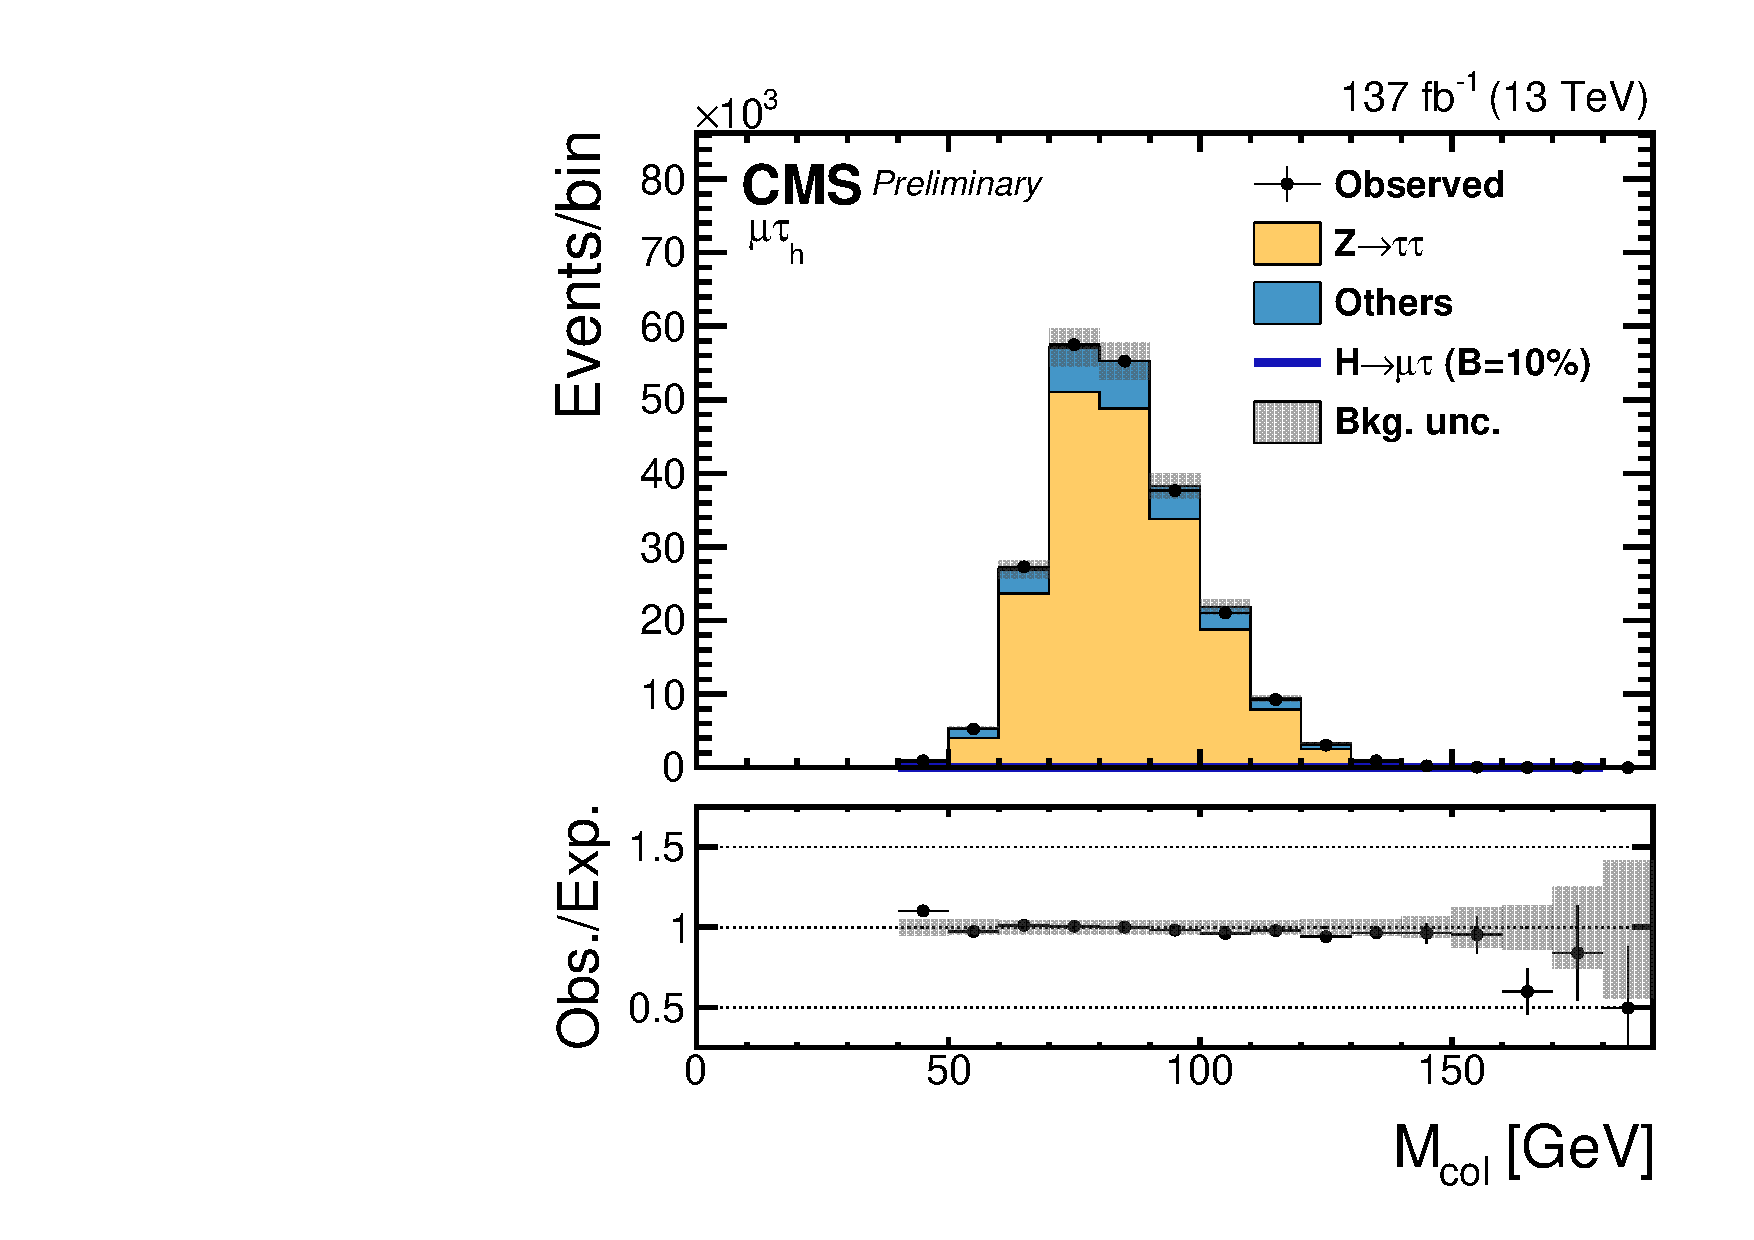
\includegraphics[width=0.45\textwidth]{plots/chapter7/Fake/mutau/ZTT.pdf}}
  \subfigure[]{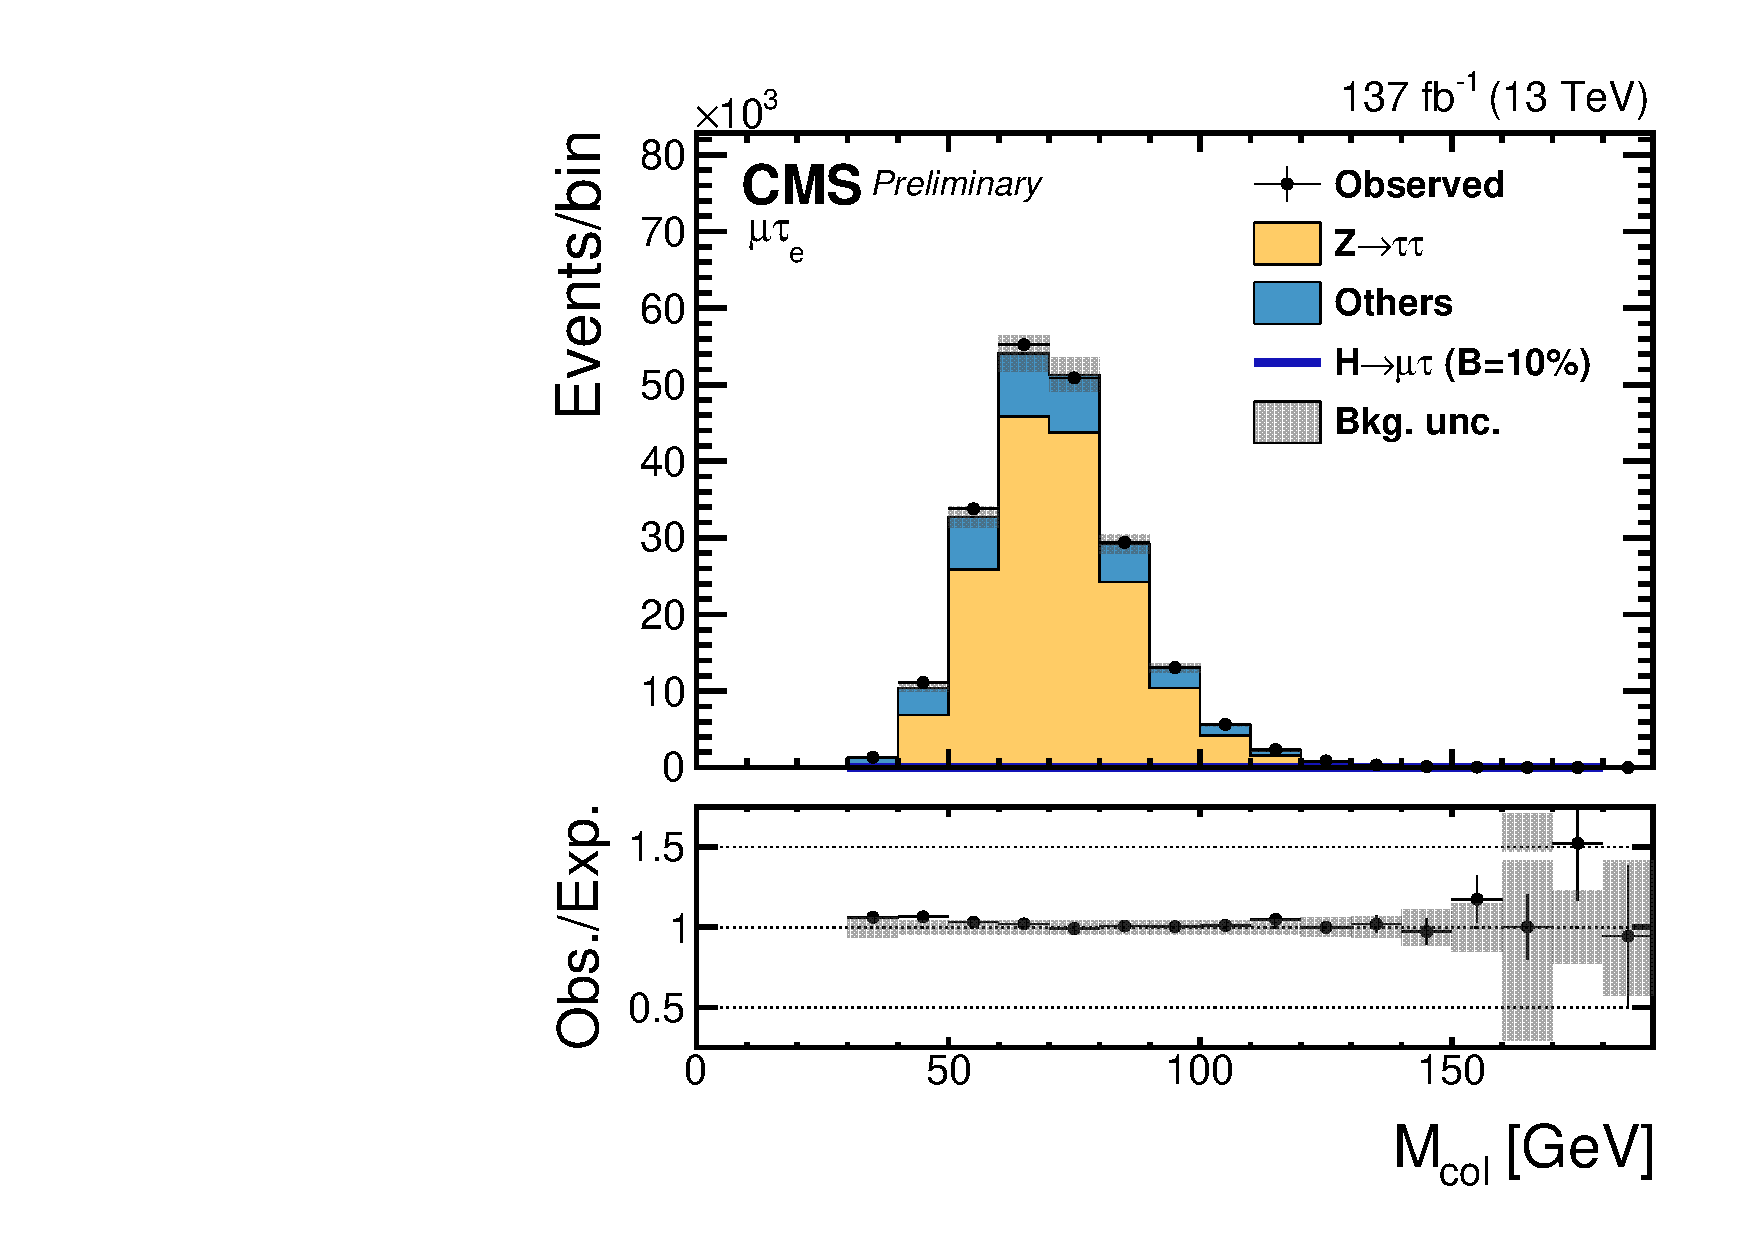
\includegraphics[width=0.45\textwidth]{plots/chapter7/Fake/mue/ZTT.pdf}}
  \subfigure[]{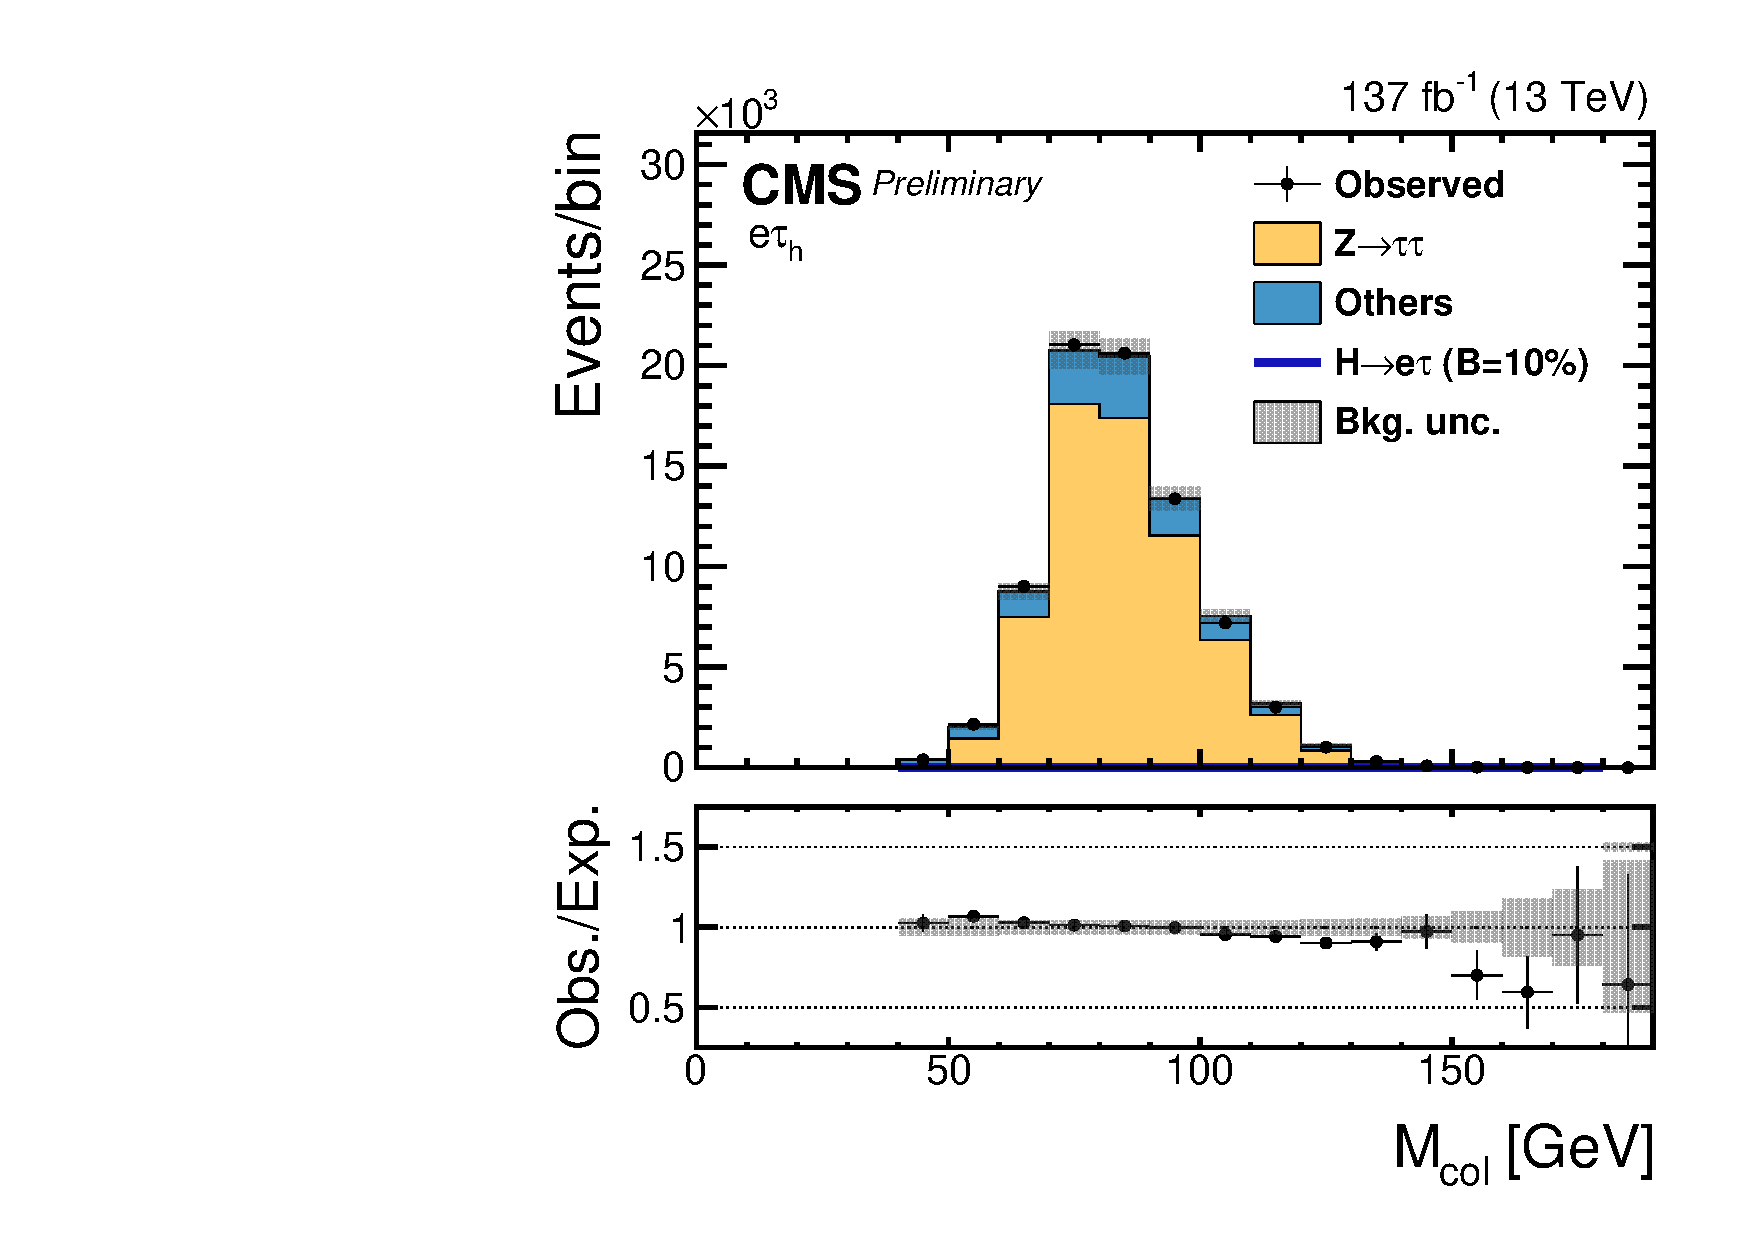
\includegraphics[width=0.45\textwidth]{plots/chapter7/Fake/etau/ZTT.pdf}}
  \subfigure[]{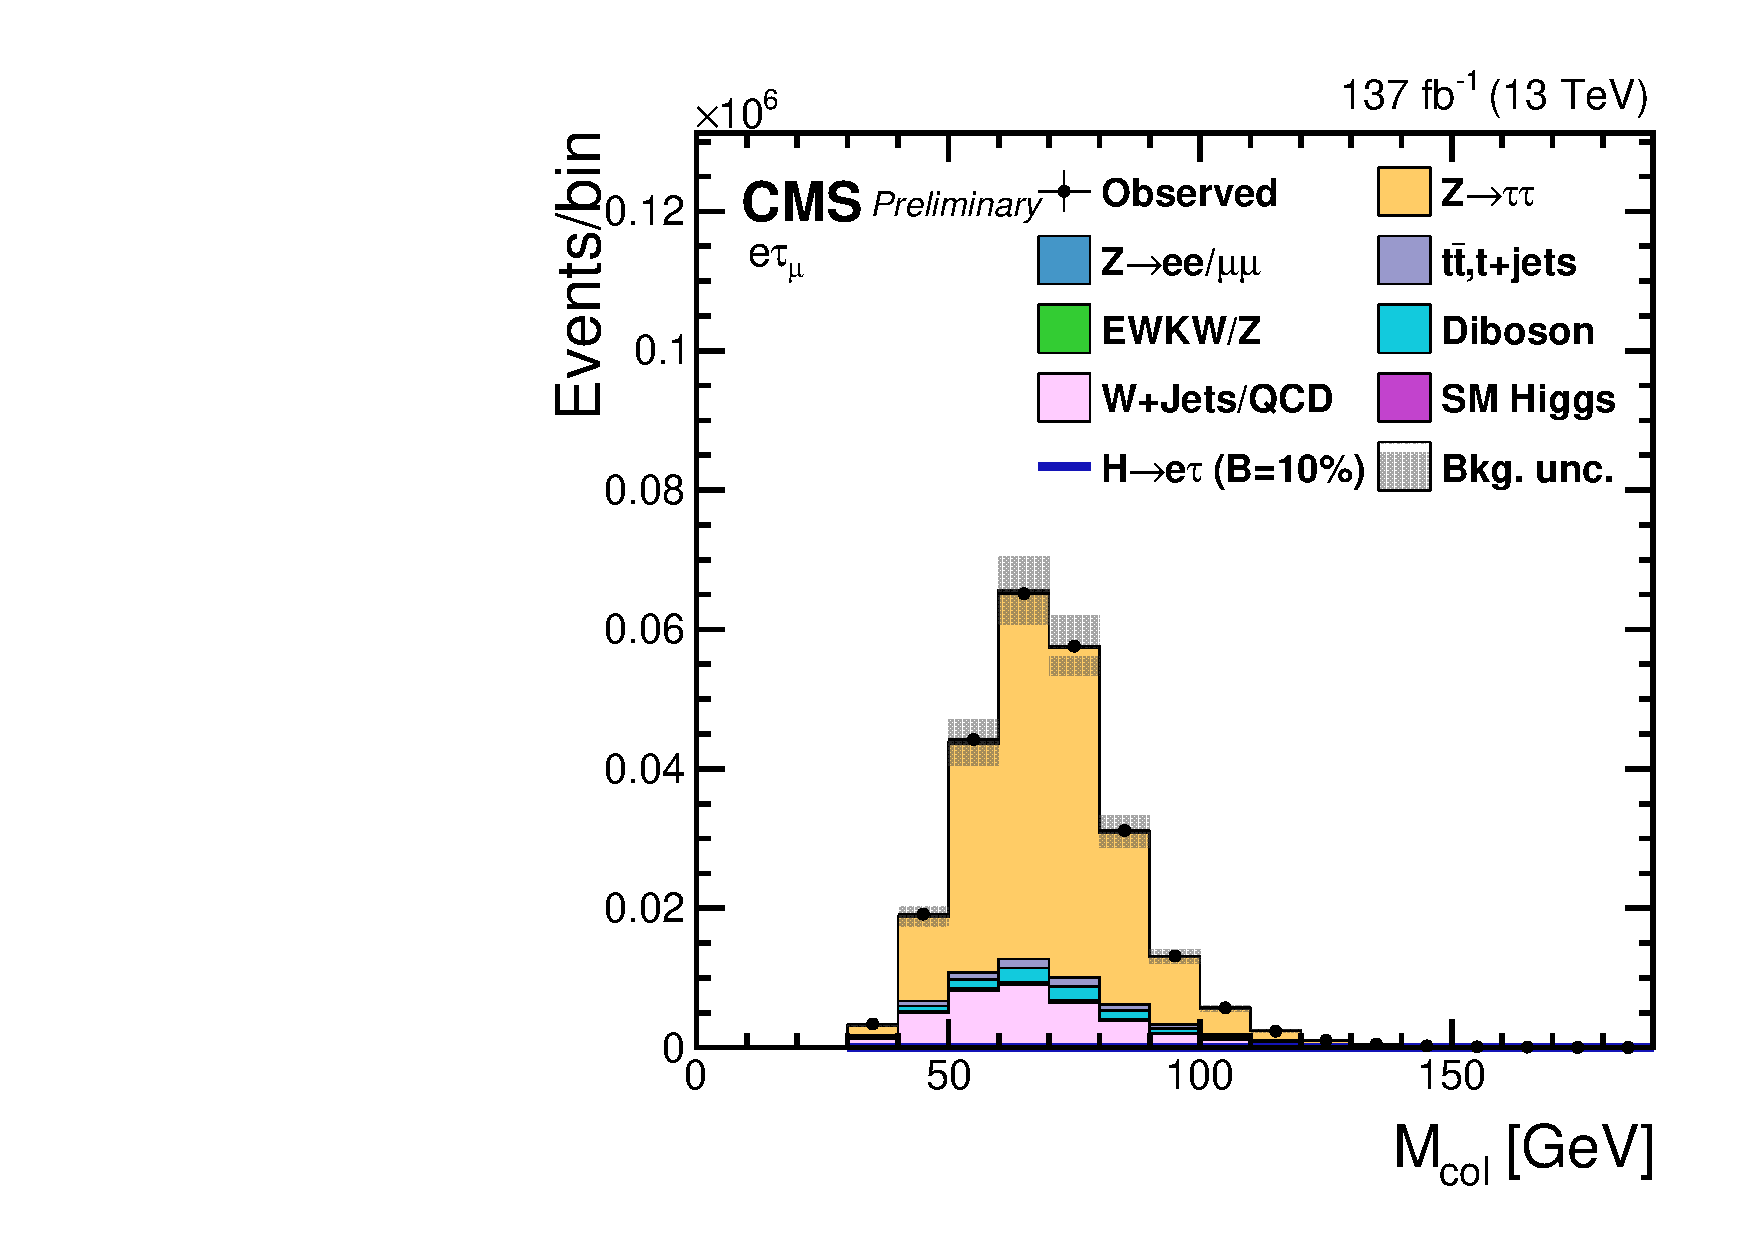
\includegraphics[width=0.45\textwidth]{plots/chapter7/Fake/emu/ZTT.pdf}}
  \caption{Distributions of \mcol discriminator in the \Ztt control regions for the (a) \muhad, (b) \mue, (c) \ehad, and (d) \emu channels.}
  \label{fig:ztt_control}
\end{figure}

\begin{figure}[htbp!]
  \centering
  \subfigure[]{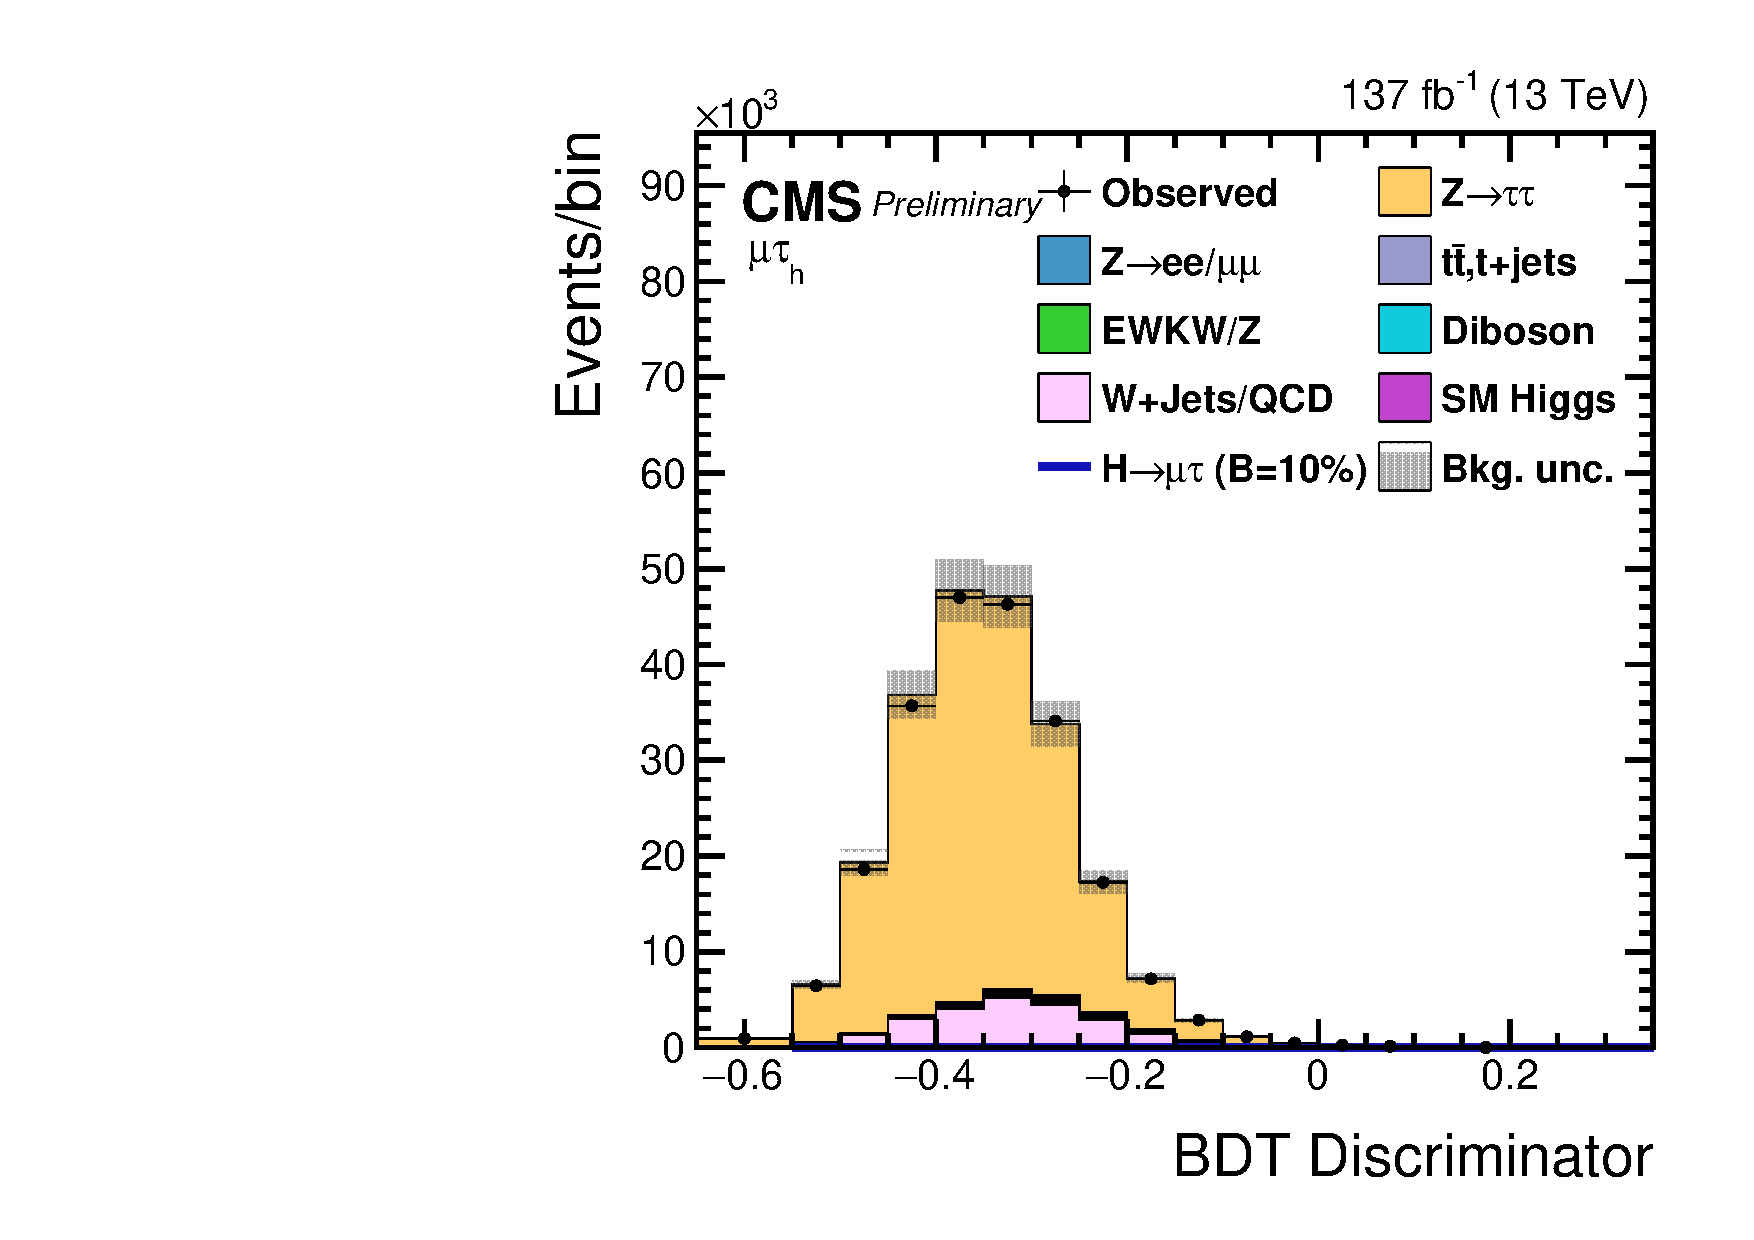
\includegraphics[width=0.45\textwidth]{plots/chapter7/Fake/mutau/ZTTBDT.pdf}}
  \subfigure[]{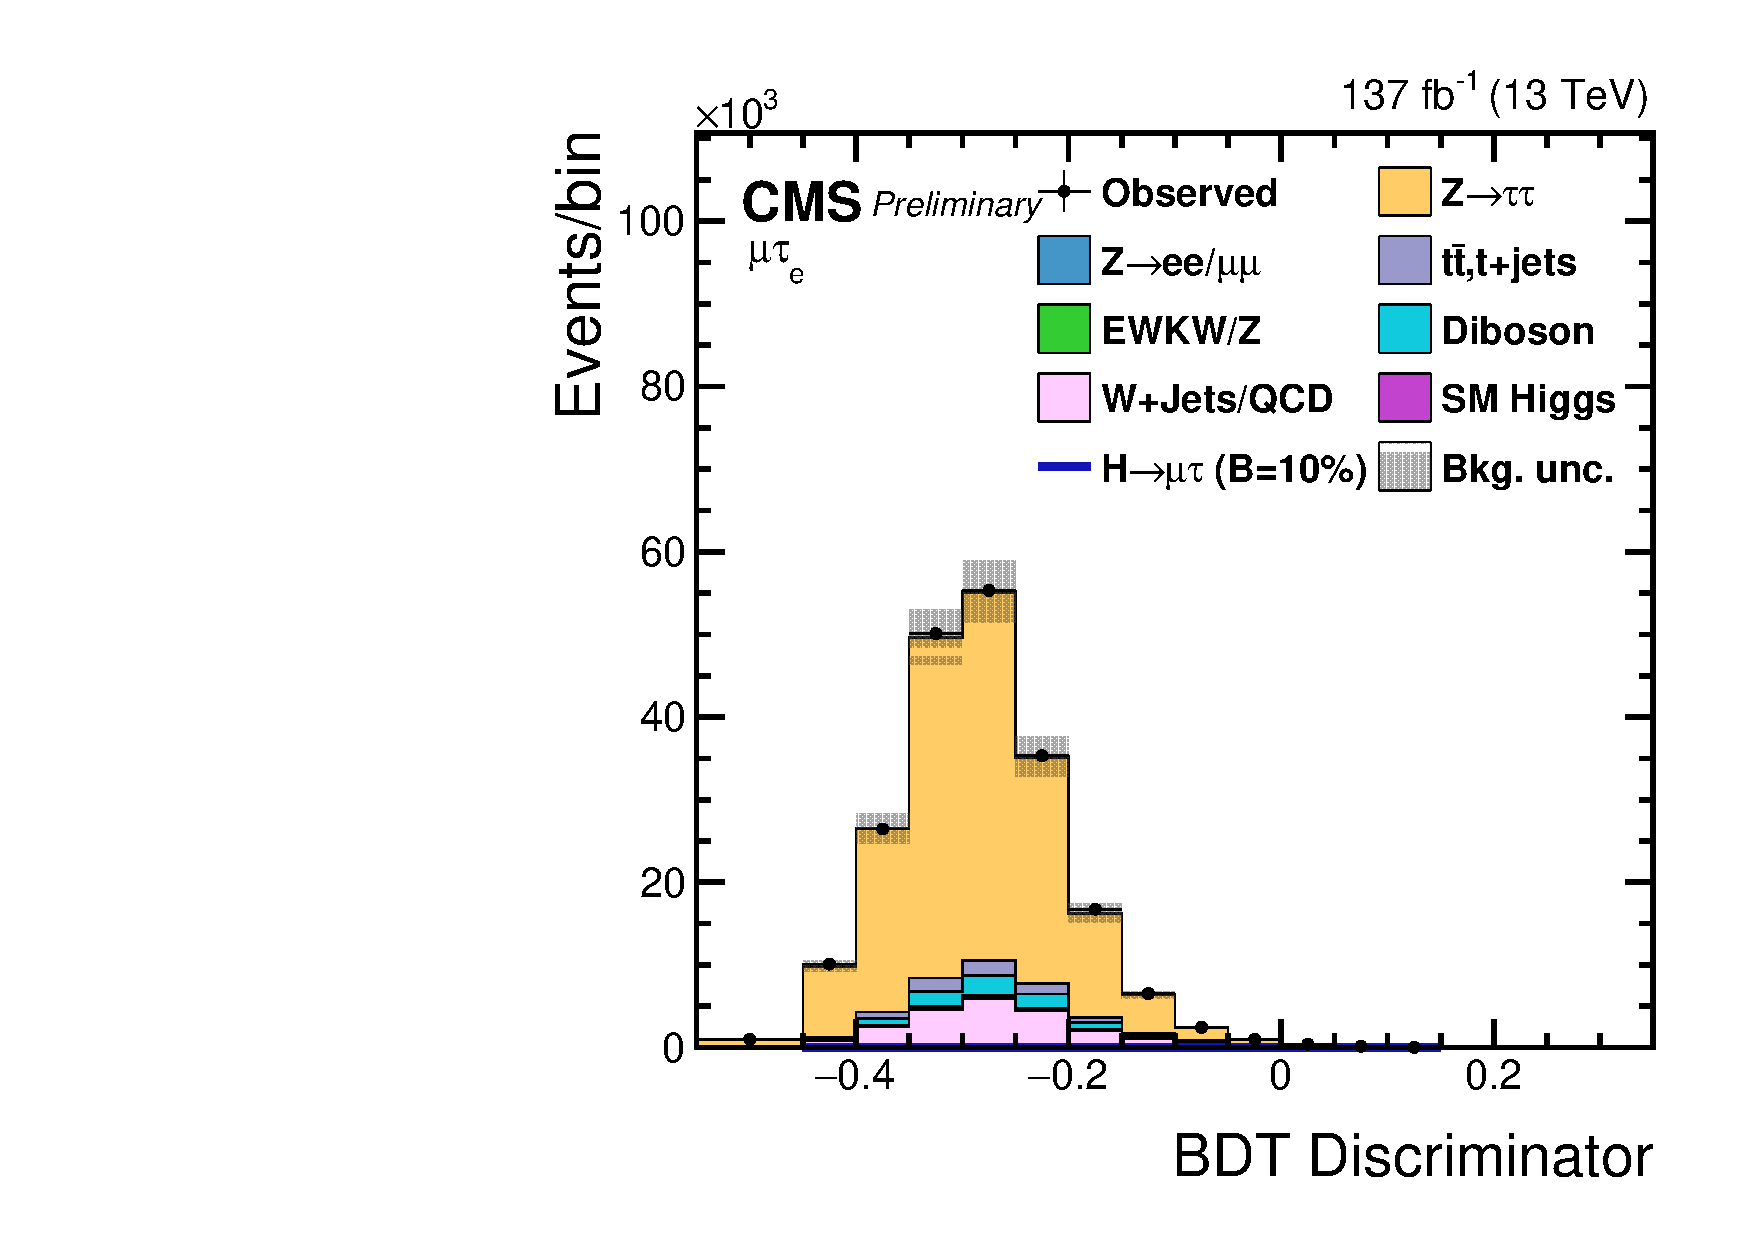
\includegraphics[width=0.45\textwidth]{plots/chapter7/Fake/mue/ZTTBDT.pdf}}
  \subfigure[]{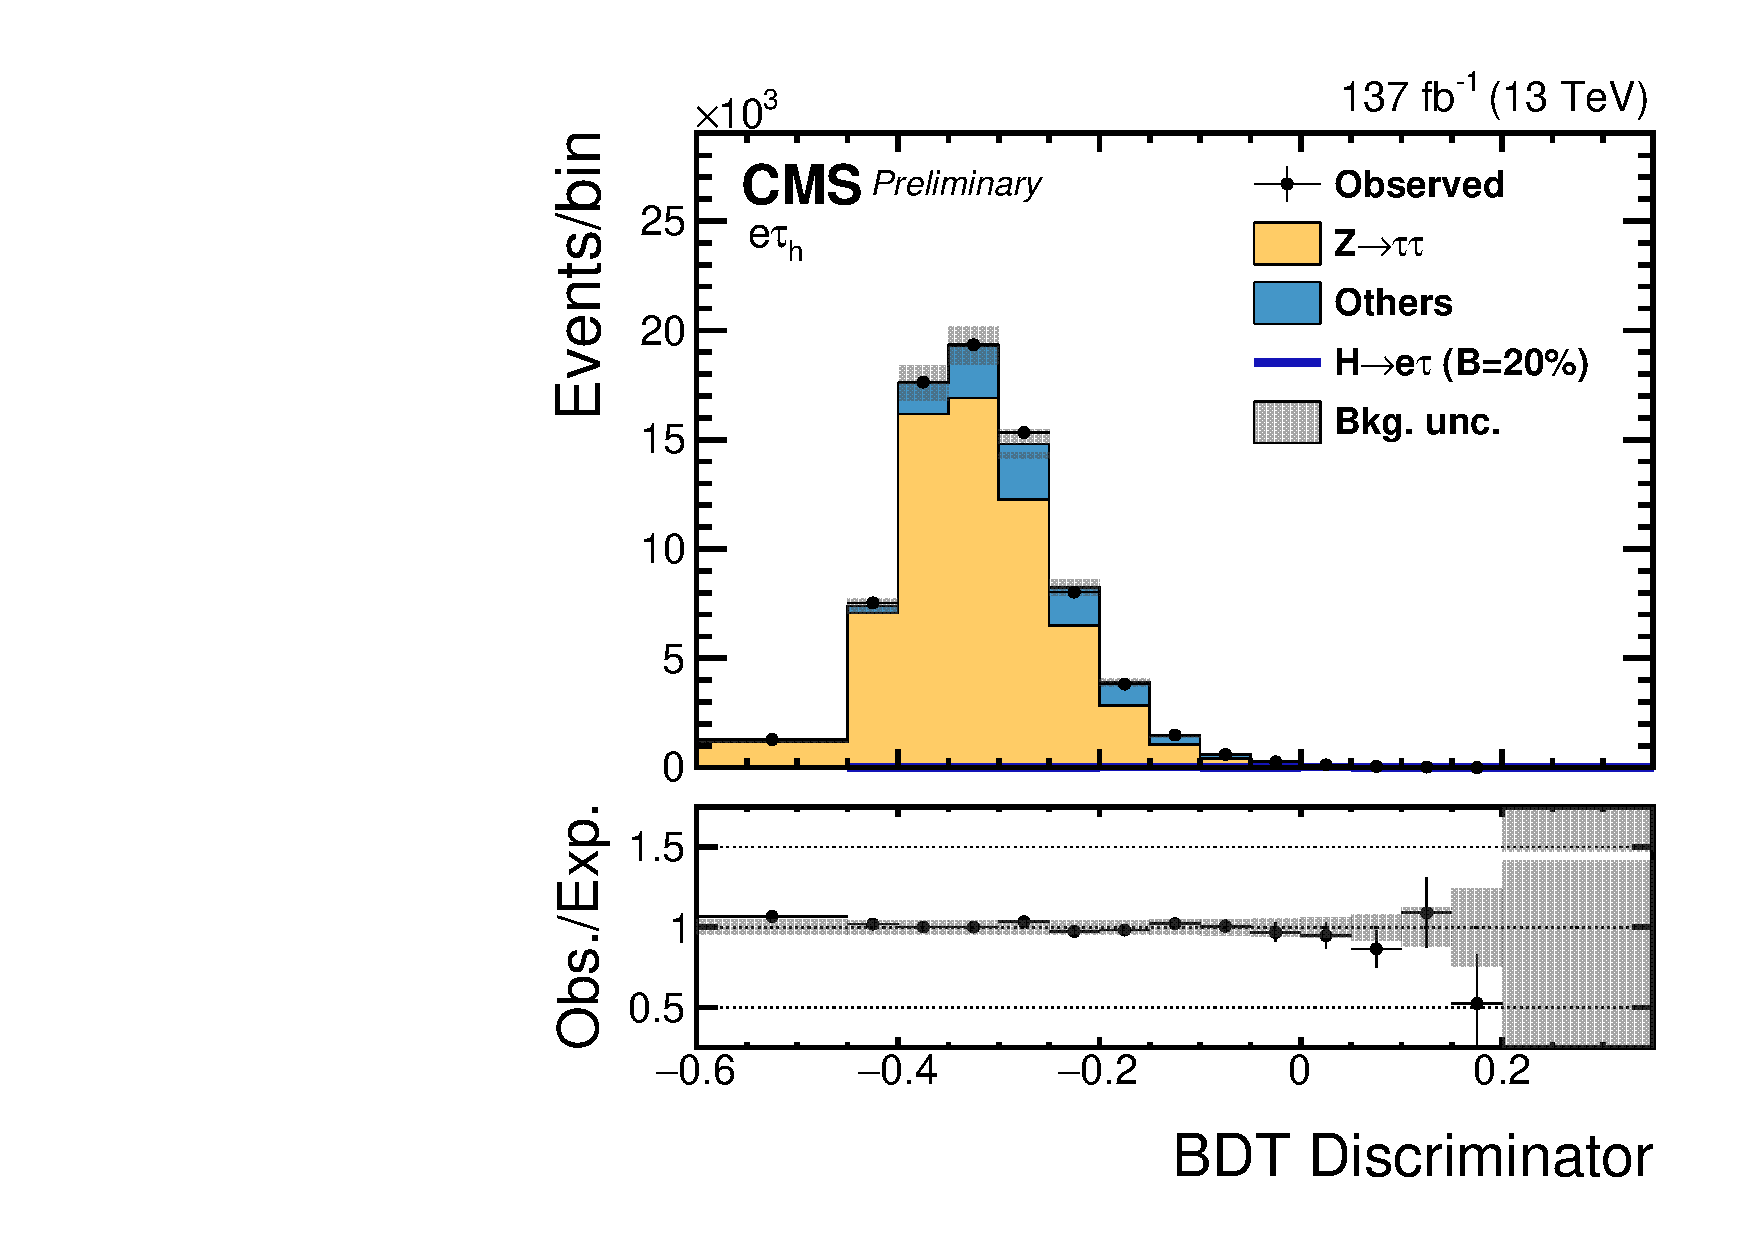
\includegraphics[width=0.45\textwidth]{plots/chapter7/Fake/etau/ZTTBDT.pdf}}
  \subfigure[]{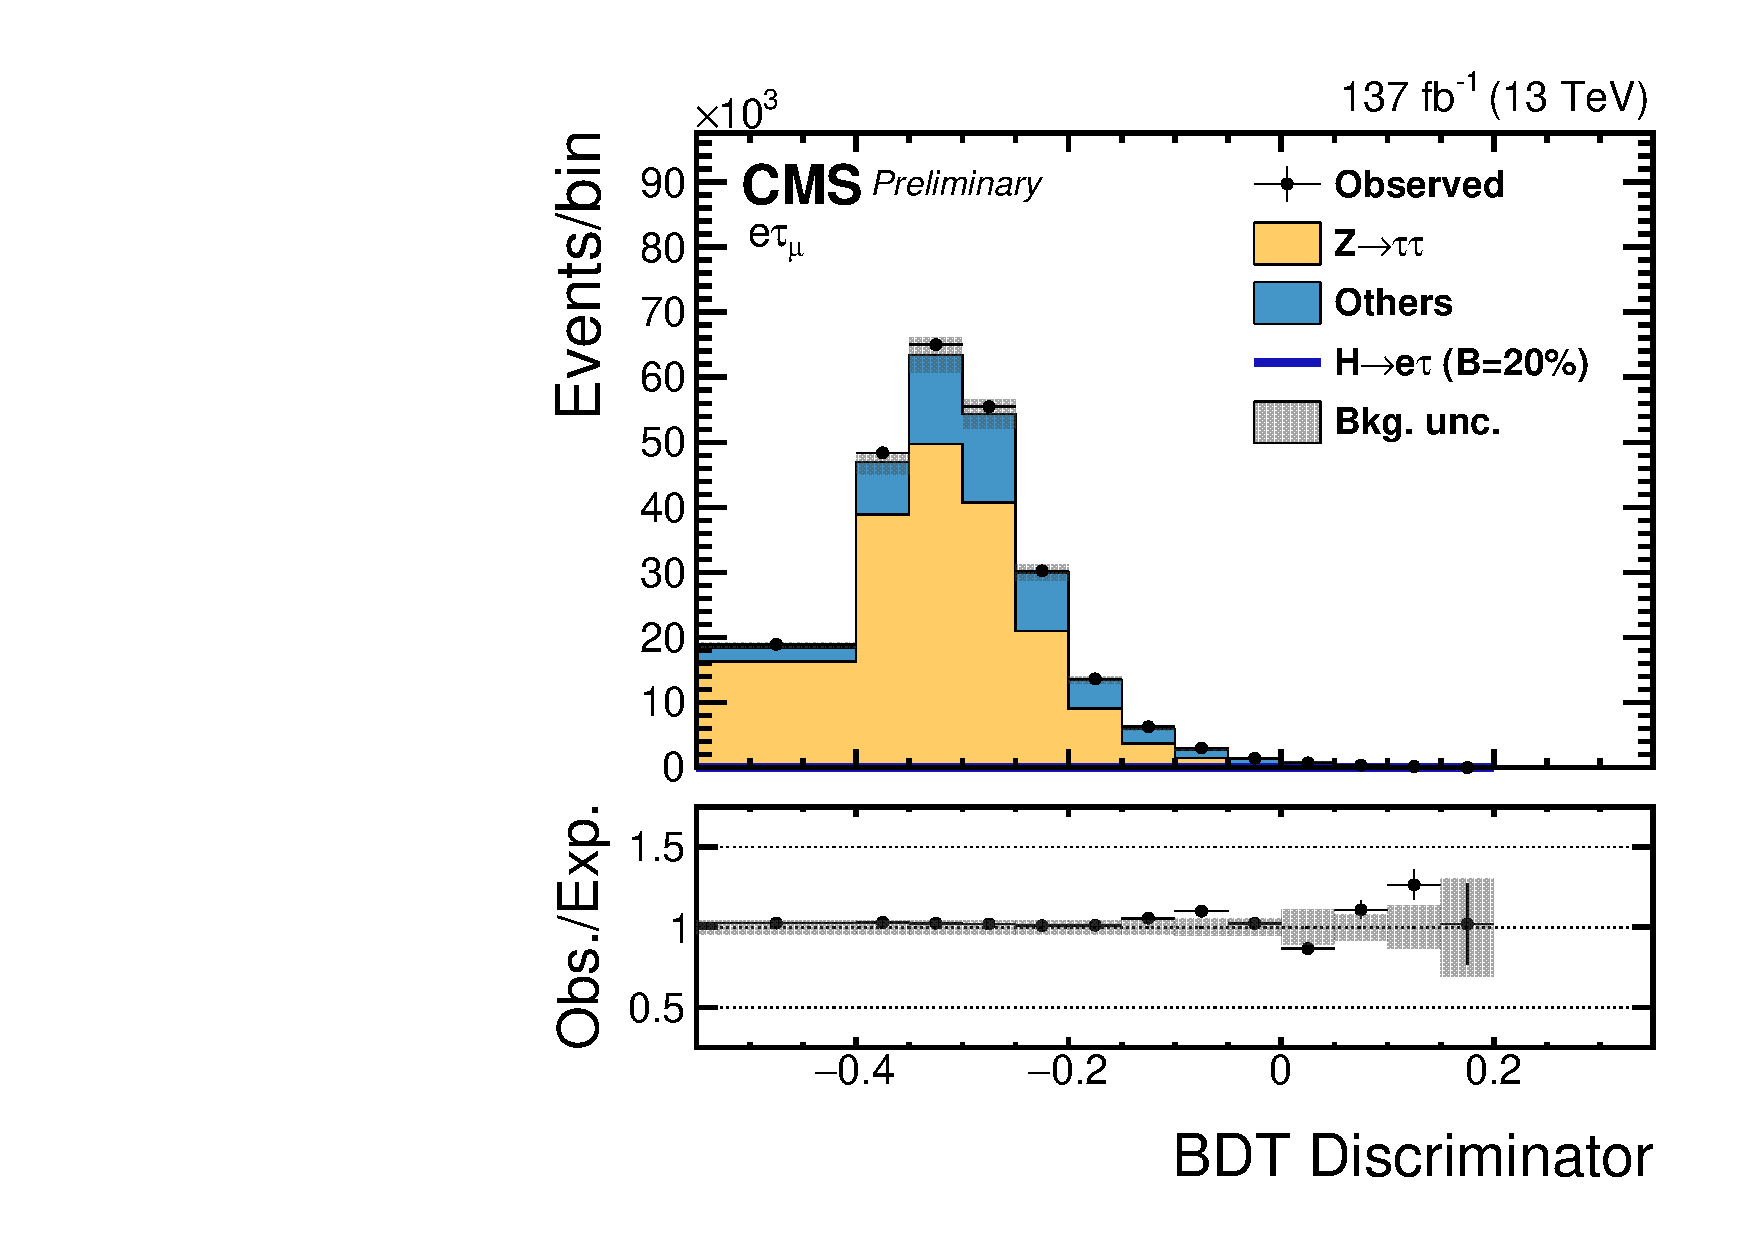
\includegraphics[width=0.45\textwidth]{plots/chapter7/Fake/emu/ZTTBDT.pdf}}
  \caption{Distributions of BDT discriminator in the \Ztt control regions for the (a) \muhad, (b) \mue, (c) \ehad, and (d) \emu channels.}
  \label{fig:ztt_control_BDT}
\end{figure}

\section{Misidentified lepton background}
The misidentified lepton background corresponds to processes where jets are misidentified as leptons. They mostly arise from two sources, \wjets, and QCD multijet events. In \wjets background events, one of the lepton candidates is from the \PW boson decay while the other is a jet misidentified as a lepton. In QCD multijet events, both the lepton candidates are misidentified jets. In two channels of this analysis (\muhad and \ehad), the contributions from misidentified lepton backgrounds have been estimated using a fully data-driven approach. In the leptonic channels (\mue and \emu), a semi data-driven approach is adopted. The semi data-driven approach results are consistent with the fully data-driven method and are undertaken due to limited statistics in the leptonic channel.

\subsection{Fully data-driven approach}
The misidentified lepton background in the signal region is estimated using misidentification rates measured in a \zjets control region and applied to a background enriched sample from collision data. The misidentification rates are evaluated using events with a \PZ boson candidate and at least one jet that can be misidentified as a lepton. The signal region contrasted with the background enriched regions used for determining the misidentified background can be seen in Figure~\ref{fig:fake}.

\begin{figure}[hbtp!]
  \centering
  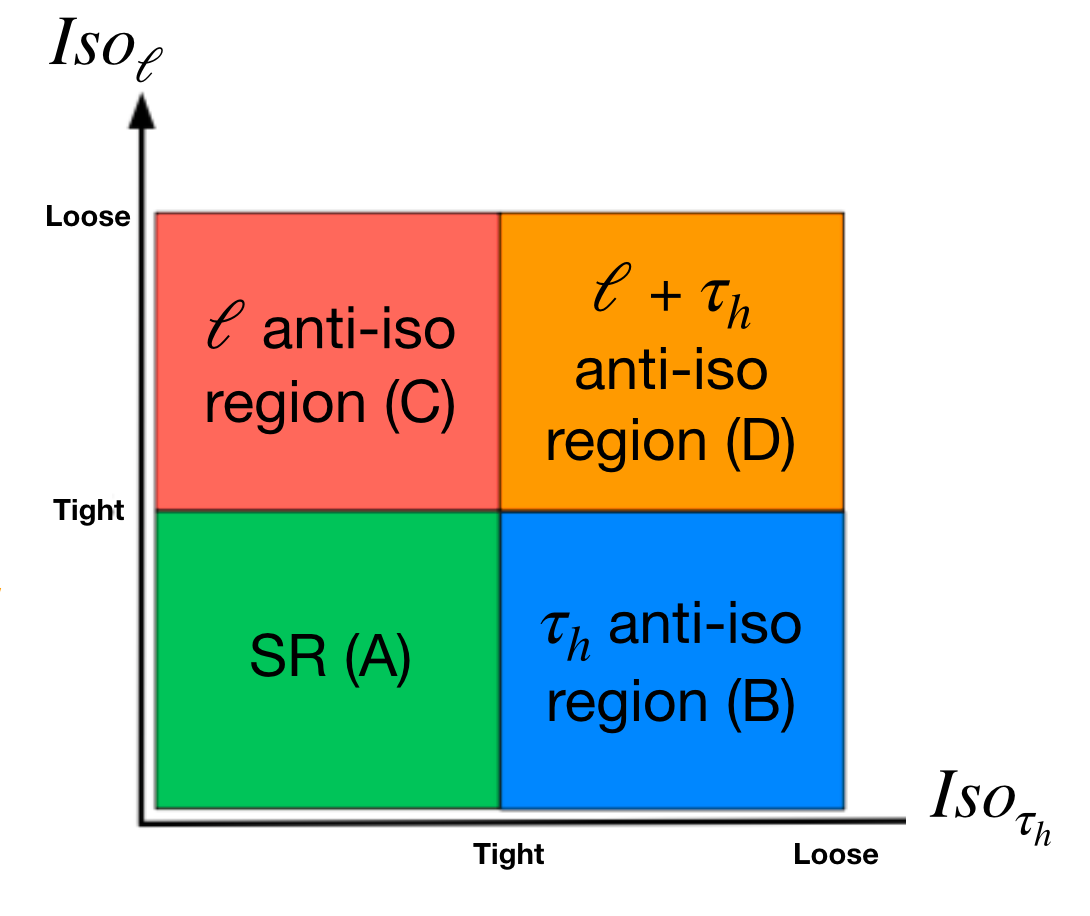
\includegraphics[width=0.49\textwidth]{plots/chapter7/Fake/Fake.png}
  \caption{Signal region (green) contrasted with the background enriched regions used for estimating the misidentified background}
  \label{fig:fake}
\end{figure}

The probabilities with which jets are misidentified as an electron, muon, or \tauh are labeled as $f_\Pe, f_\Pgm$, and $f_{\tauh}$, respectively. The \PZ boson candidate is formed using two muons with $\pt > 26 \GeV$ and $\aeta < 2.4$ and $\irel < 0.15$ for measuring the jet $\to\tauh, \Pgm, \Pe$ misidentification rate. The muons are required to be oppositely charged and have their invariant mass between 70 and 110~\GeV. The contribution from diboson events, where the jet candidate corresponds to a real lepton, is subtracted using simulation. The jet is required to pass the same lepton identification criteria as used in the SR. A ``signal-like'' sample is defined if the jet passes the tight lepton isolation, otherwise a ``background-like'' sample is defined if it only passes the looser lepton isolation. These two samples are used to estimate $f_\Pe, f_\Pgm,$ and $f_{\tauh}$ following:
\begin{linenomath*}
  \begin{equation*}
    f_{i} = \frac{N_i(\text{signal-like})}{N_{i}(\text{background-like}) + N_i(\text{signal-like})}
  \end{equation*}
\end{linenomath*}
where $N_i(\text{signal-like})$ is the number of events with a third lepton candidate that passes the tight lepton isolation, while $N_i(\text{background-like})$ is the number of events that pass only the looser lepton isolation and index $i = \Pe, \Pgm,$ or \Pgt.

As can be seen in tables~\ref{tab:mutau_evtselection} and~\ref{tab:etau_evtselection}, the isolation for the electron and the muon is required to be $\irel < 0.15$ and the \tauh is discriminated against jets with a WP that has an identification efficiency of about 70\% for ``signal-like'' sample. For the ``background-like'' sample, lepton isolation is required to be $0.15 < \irel < 0.25$ for the muon, $0.15 < \irel < 0.5$ for the electron, and the \tauh is discriminated against jets with a WP that has an identification efficiency of about $\sim 80\%$ and not pass the ``signal-like'' WP. After the ``signal-like'' and ``background-like'' samples are defined the misidentification rates are computed as a function of the lepton \pt. The \tauh misidentification rate shows a \pt dependence that varies with the \tauh decay mode and \aeta and are thus evaluated as a function of $\pt^{\Pgt}$ for the different decay modes and two \aeta regions ($\aeta < 1.5$ or $\aeta > 1.5$).

In the \ehad channel, the \tauh misidentification rate is evaluated using events with a \PZ boson candidate that decays into two electrons with $\pt > 27 \GeV$ and $\aeta < 2.5$ and $\irel < 0.15$. The electrons must be oppositely charged and have their invariant mass between 70 and 110~\GeV. The reason for using \Zee events for evaluating the \tauh misidentification rate in \ehad channel is that the DNN WPs used for discriminating \tauh against electrons and muons are different in this channel compared to the \muhad channel. The misidentification rates evaluated using this control region are compatible with the misidentification rates measured in \Zmm events. The electron, muon, and \tauh misidentification rates can be seen in Figure~\ref{fig:fakerate_tauh} and~\ref{fig:fakerate_lepton}.

\begin{figure}[htbp]
  \centering
  \subfigure[]{
    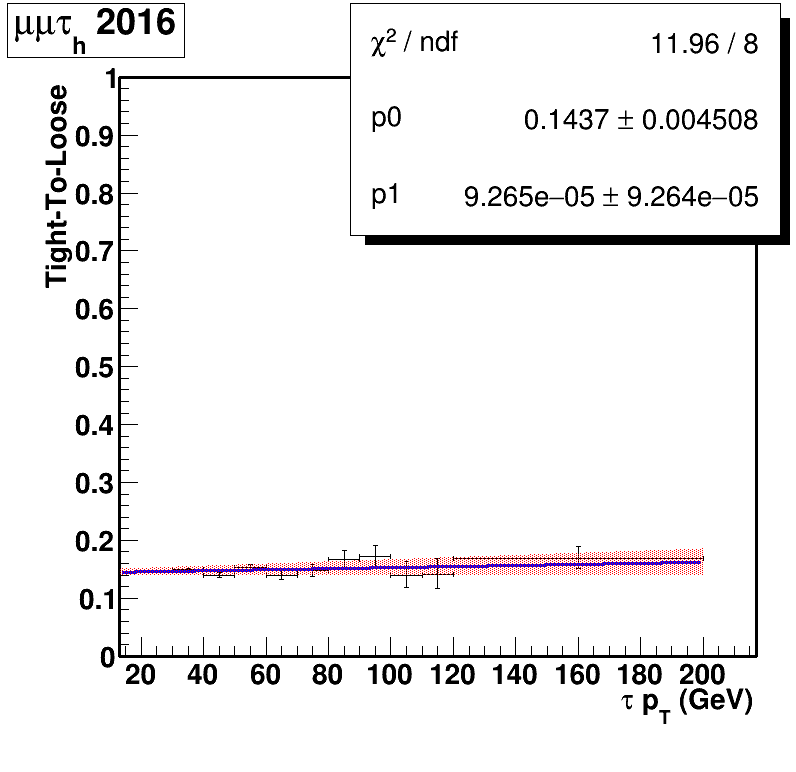
\includegraphics[width=0.3\textwidth]{plots/chapter7/Fake/FR/MMT2016.png}
    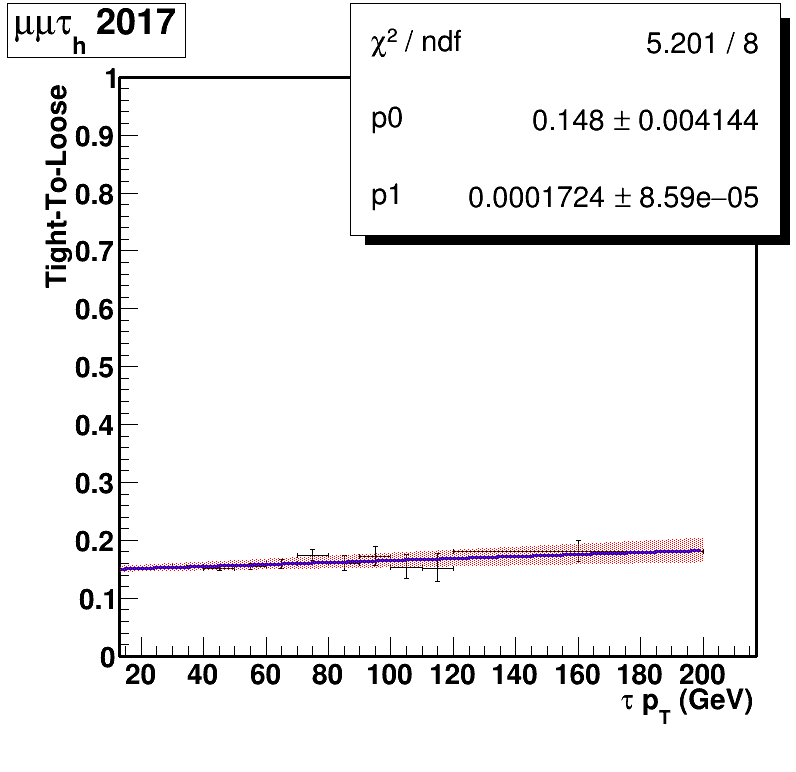
\includegraphics[width=0.3\textwidth]{plots/chapter7/Fake/FR/MMT2017.png}
    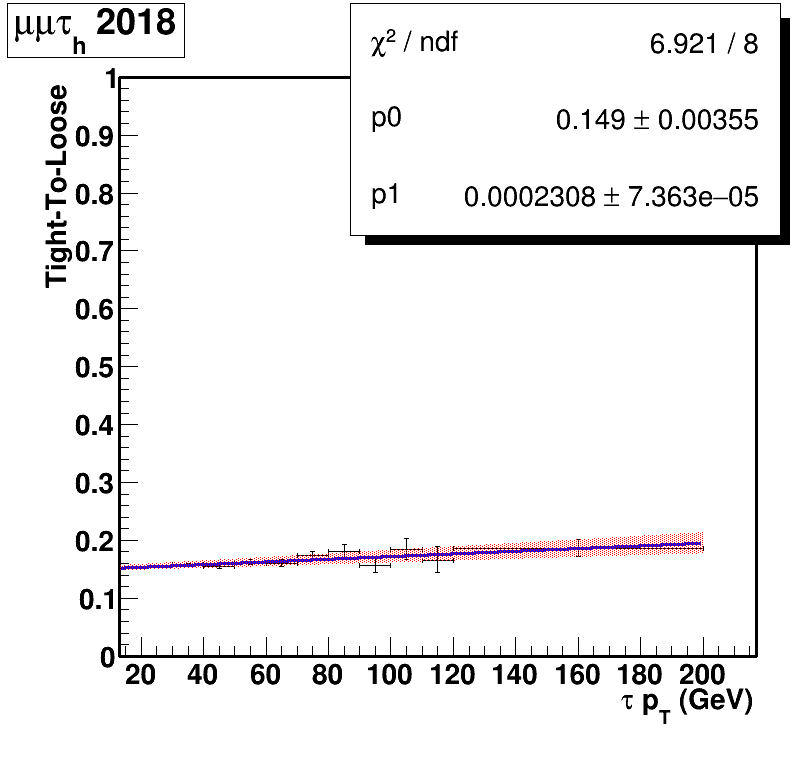
\includegraphics[width=0.3\textwidth]{plots/chapter7/Fake/FR/MMT2018.png} electron
  }
  \subfigure[]{
    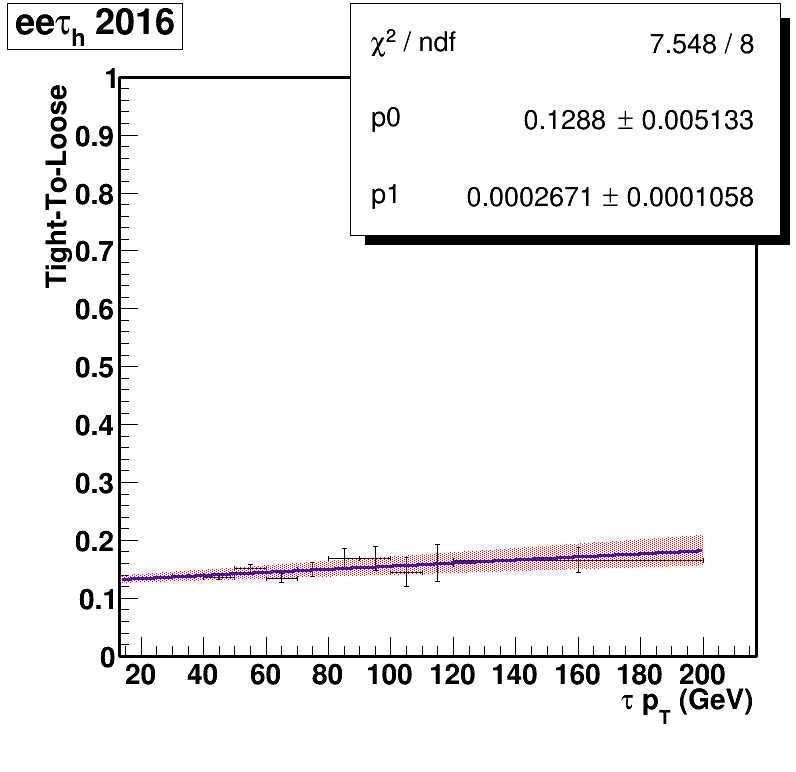
\includegraphics[width=0.3\textwidth]{plots/chapter7/Fake/FR/EET2016.png}
    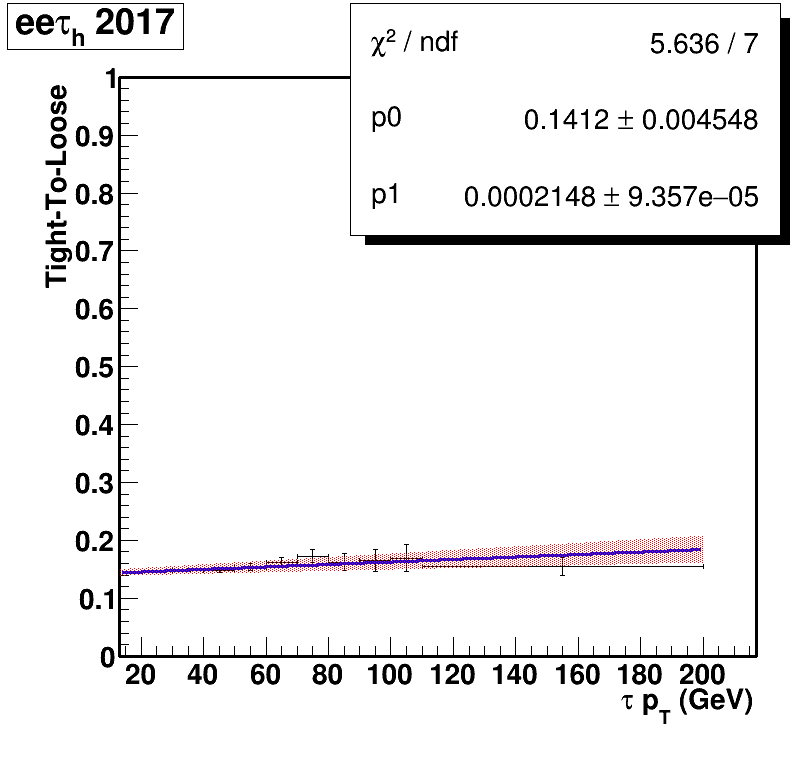
\includegraphics[width=0.3\textwidth]{plots/chapter7/Fake/FR/EET2017.png}
    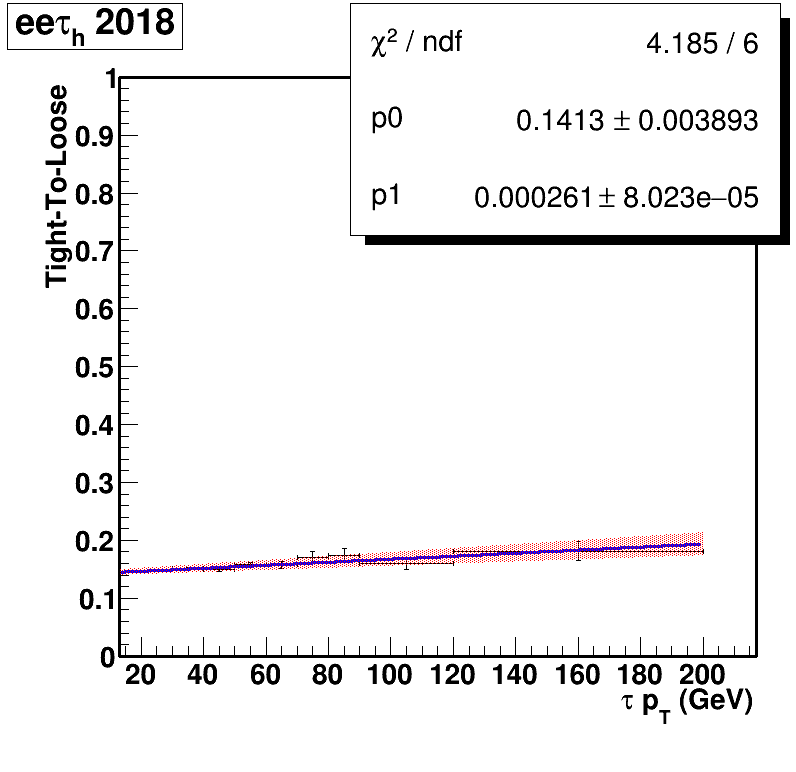
\includegraphics[width=0.3\textwidth]{plots/chapter7/Fake/FR/EET2018.png}
  }
  \caption{Fit performed to \tauh misidentification rates for \muhad (a) and \ehad (b) channel as a function of \tauh \pt for the different years. The misidentification rates used are further parametrized based on \tauh decay mode along with the pseudorapidity of \tauh. However, here only the inclusive misidentification rates are shown.}
  \label{fig:fakerate_tauh}
\end{figure}

\begin{figure}[htbp]
  \centering
  \subfigure[]{
    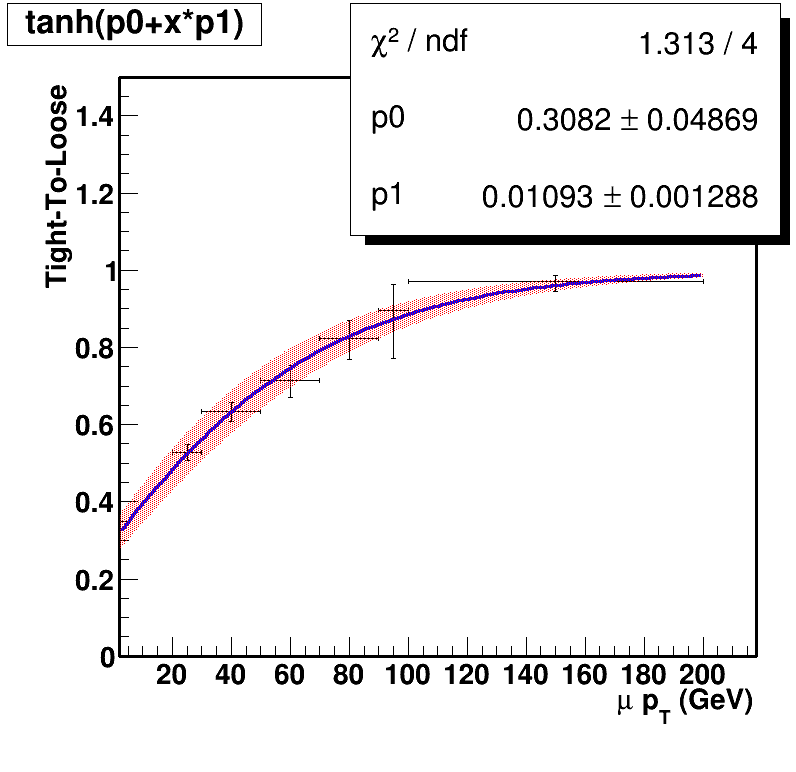
\includegraphics[width=0.3\textwidth]{plots/chapter7/Fake/FR/MMM2016.png}
    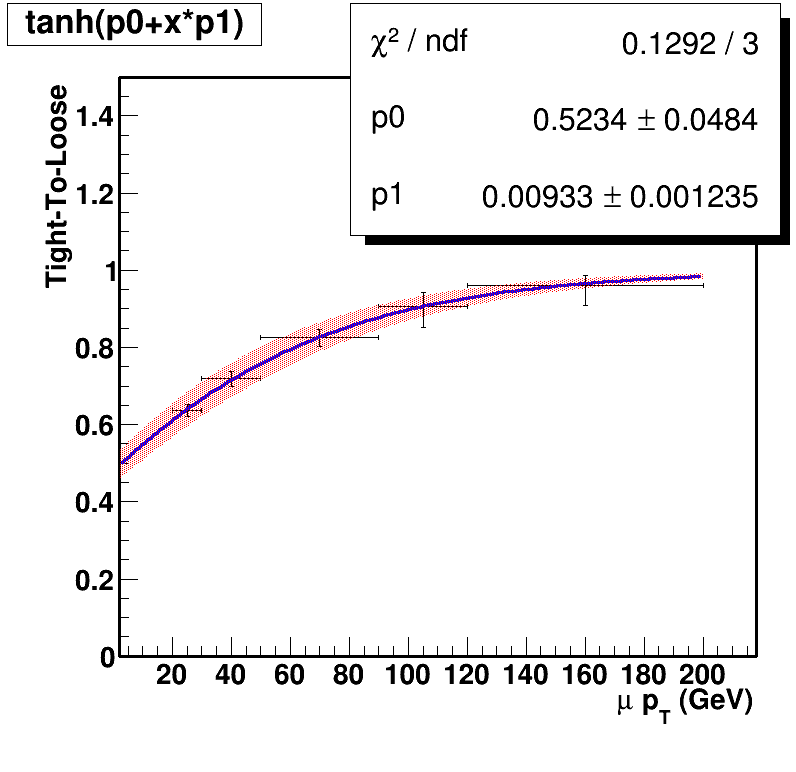
\includegraphics[width=0.3\textwidth]{plots/chapter7/Fake/FR/MMM2017.png}
    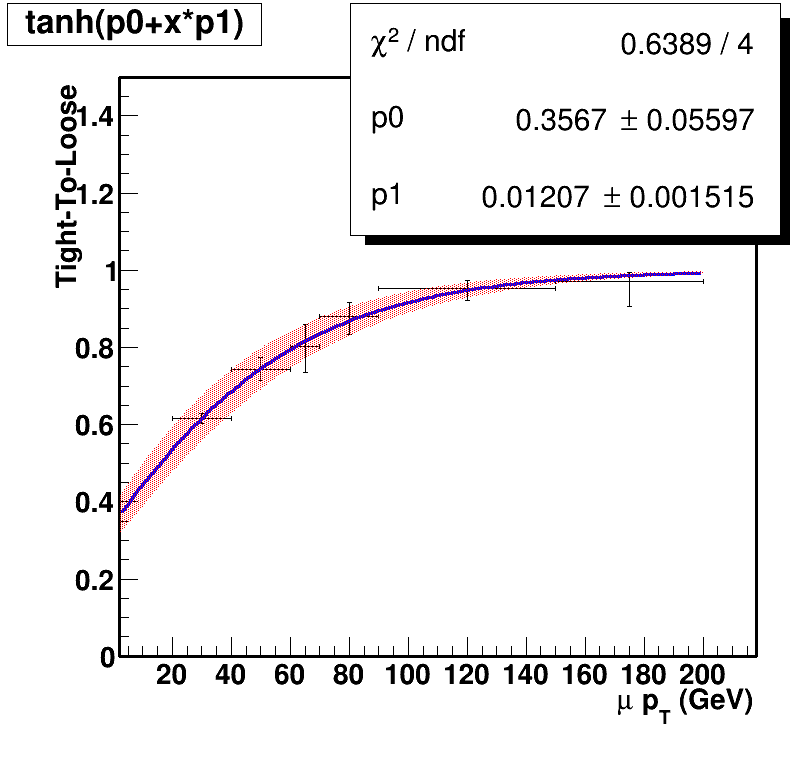
\includegraphics[width=0.3\textwidth]{plots/chapter7/Fake/FR/MMM2018.png}
  }
  \subfigure[]{
    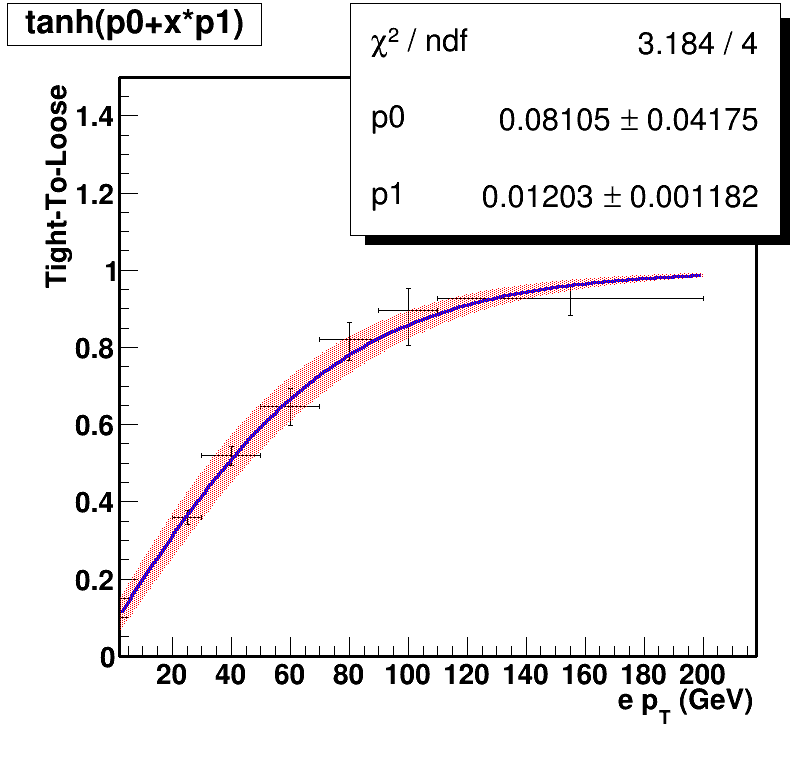
\includegraphics[width=0.3\textwidth]{plots/chapter7/Fake/FR/MME2016.png}
    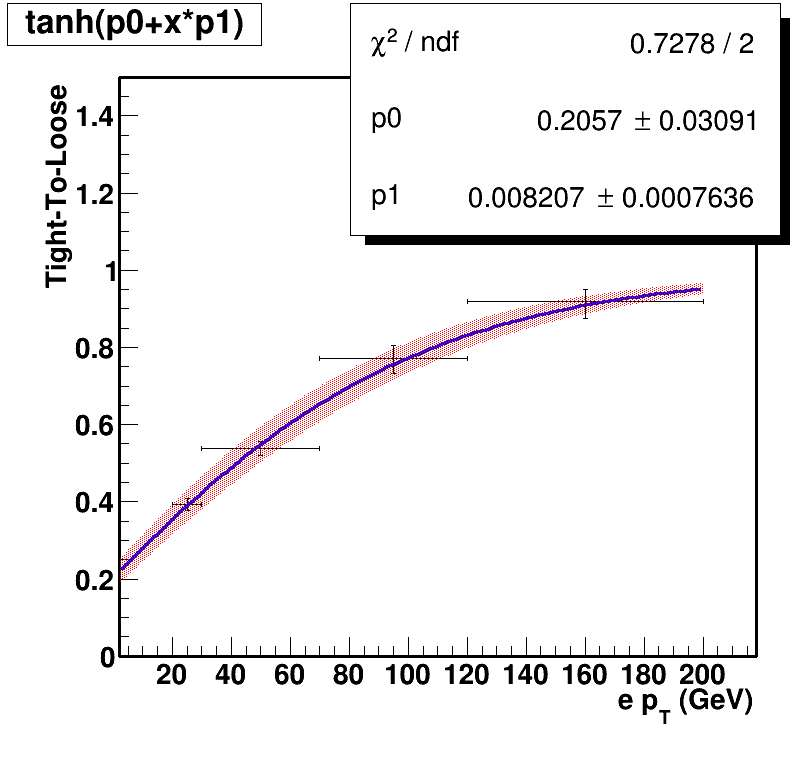
\includegraphics[width=0.3\textwidth]{plots/chapter7/Fake/FR/MME2017.png}
    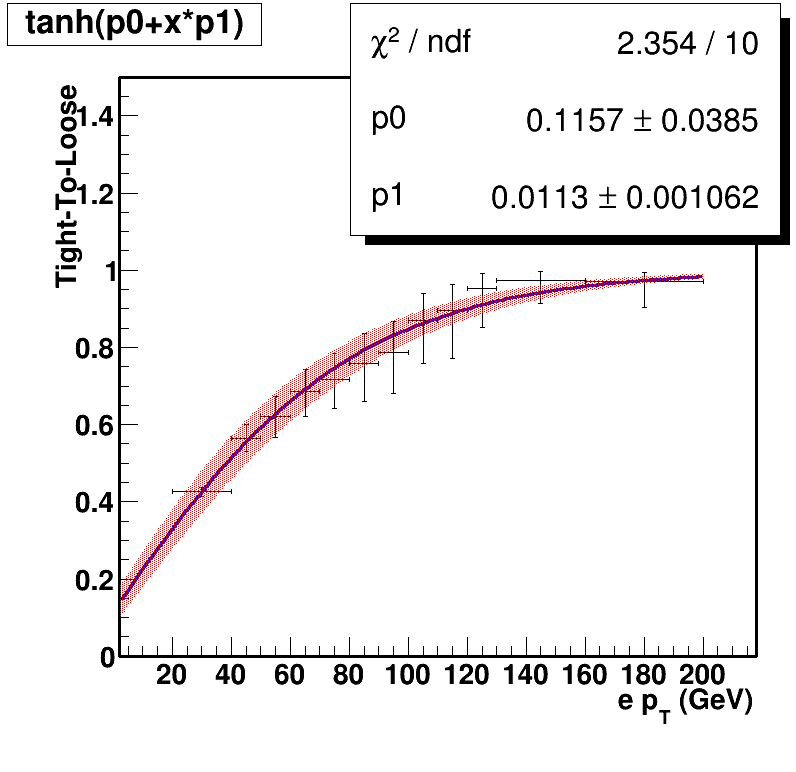
\includegraphics[width=0.3\textwidth]{plots/chapter7/Fake/FR/MME2018.png}
  }
  \caption{Fit performed to the muon (a) and electron (b) misidentification rates as a function of their \pt for 2016 (left), 2017 (center), and 2018 (right). The hyperbolic tangent function is used for performing the fit.}
  \label{fig:fakerate_lepton}
\end{figure}

Each event in the background enriched sample defined using the collision data with the same selection as the signal region, but loosening the isolation requirements on one of the leptons is then weighted by a factor $f_i/(1-f_i)$ depending on the lepton \pt for electrons and muons or \pt, $\eta$ and decay mode for the \tauh lepton candidates. Both background yields and shape distributions are thus estimated. Events with the possibility of double-counting due to two misidentified leptons are subtracted using a weight. For example, events with a misidentified muon (electron) and a misidentified \tauh are subtracted in the \muhad (\ehad) channel using a weight, $f_\Pgt f_\ell/[(1-f_\Pgt)(1-f_\ell)]$, where $\ell = \Pgm$ or \Pe.

The background estimation is validated in a control region with the same electric charge for both the leptons (same-sign), enhancing the misidentified lepton background. The misidentification rate $f_i$ is applied to events passing preselection and by inverting the lepton pair's charge requirement in both the ``background-like'' and the ``signal-like'' regions. The background estimation is also validated in a \PW boson enriched control region. This control region is obtained by applying the preselection and $\mtlmet > 60 \GeV$ ($\ell=\Pe$ or \Pgm) and $\mttmet > 80 \GeV$. The same strategy is applied in the \ehad channel, which results in a similar agreement. Figures~\ref{fig:fake_control} and~\ref{fig:fake_control_BDT} show the comparison of data with background estimates in the same sign and \PW boson enriched control regions for the \muhad and \ehad channels.

\begin{figure}[htbp!]
  \centering
  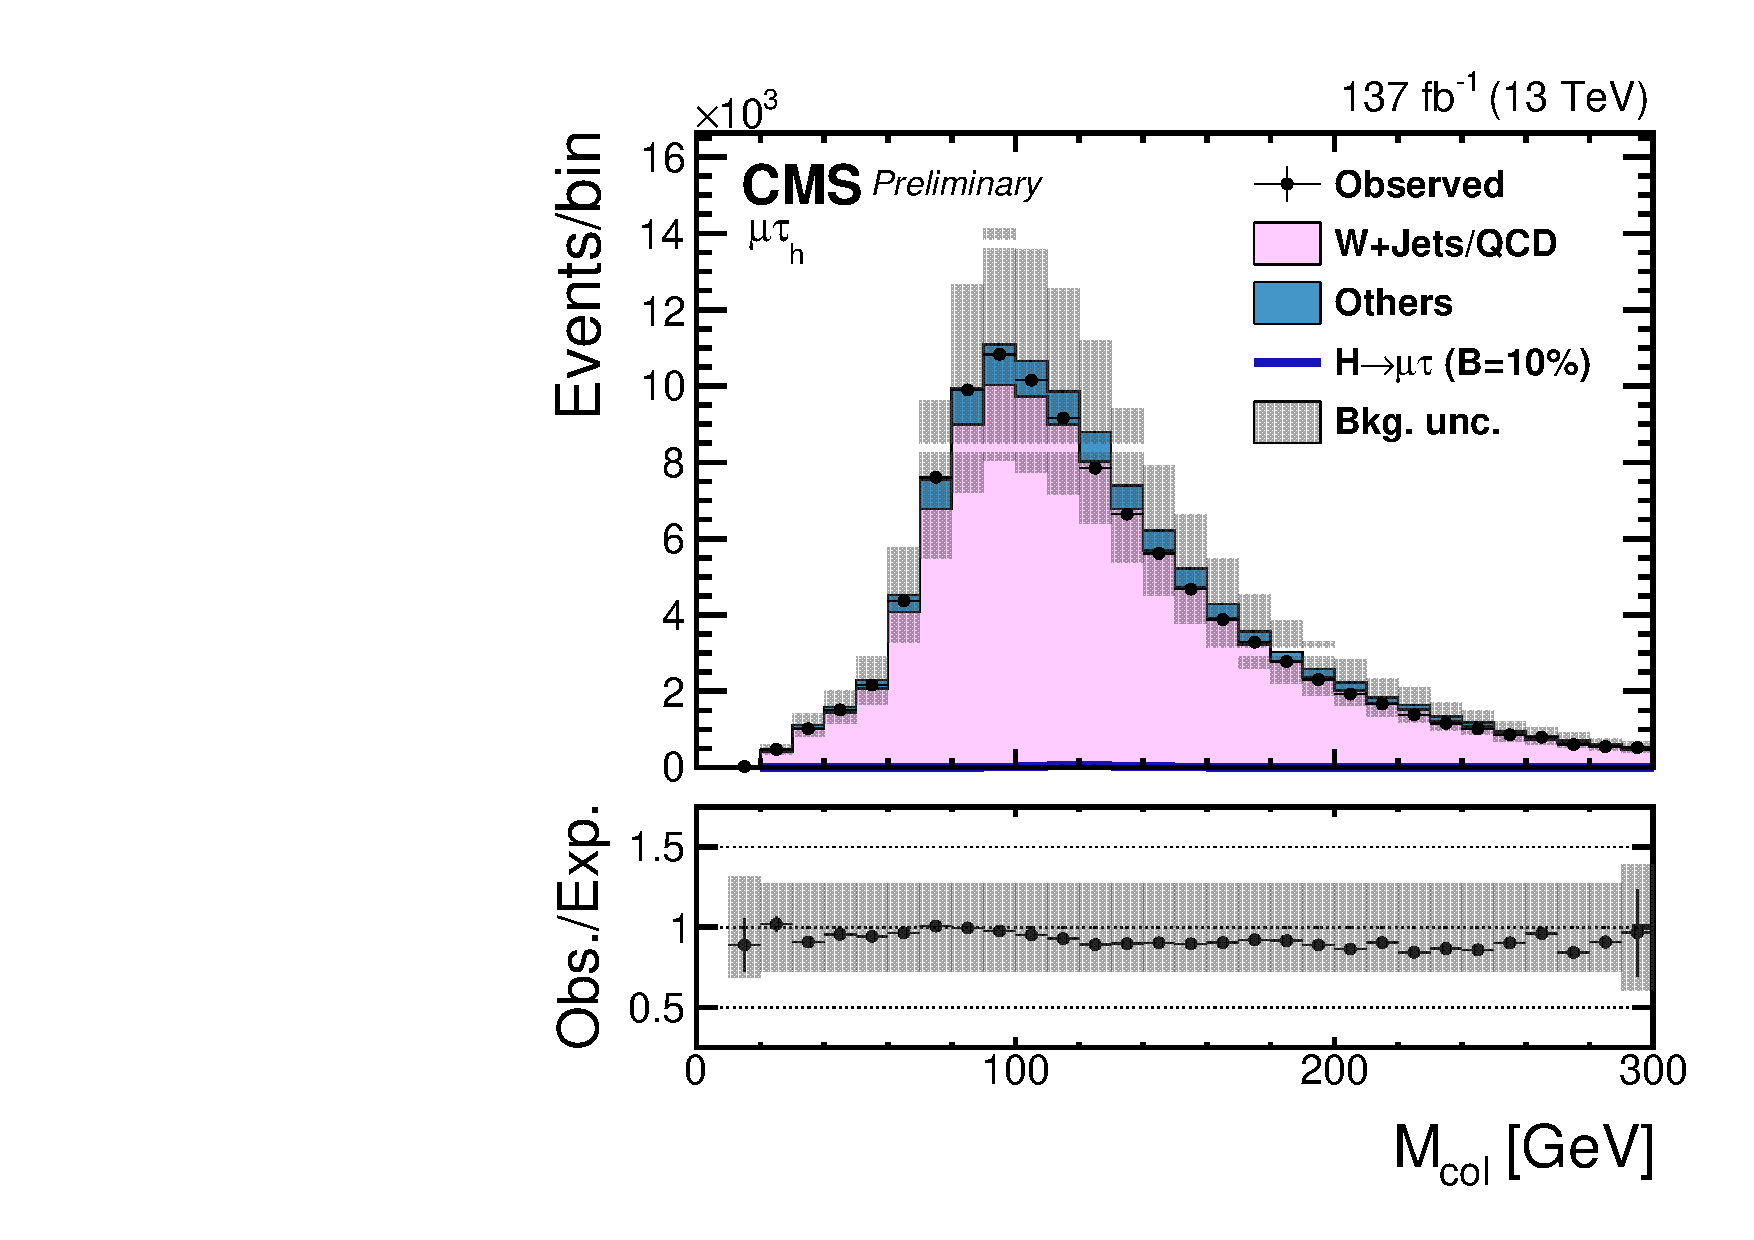
\includegraphics[width=0.45\textwidth]{plots/chapter7/Fake/mutau/SS.pdf}
  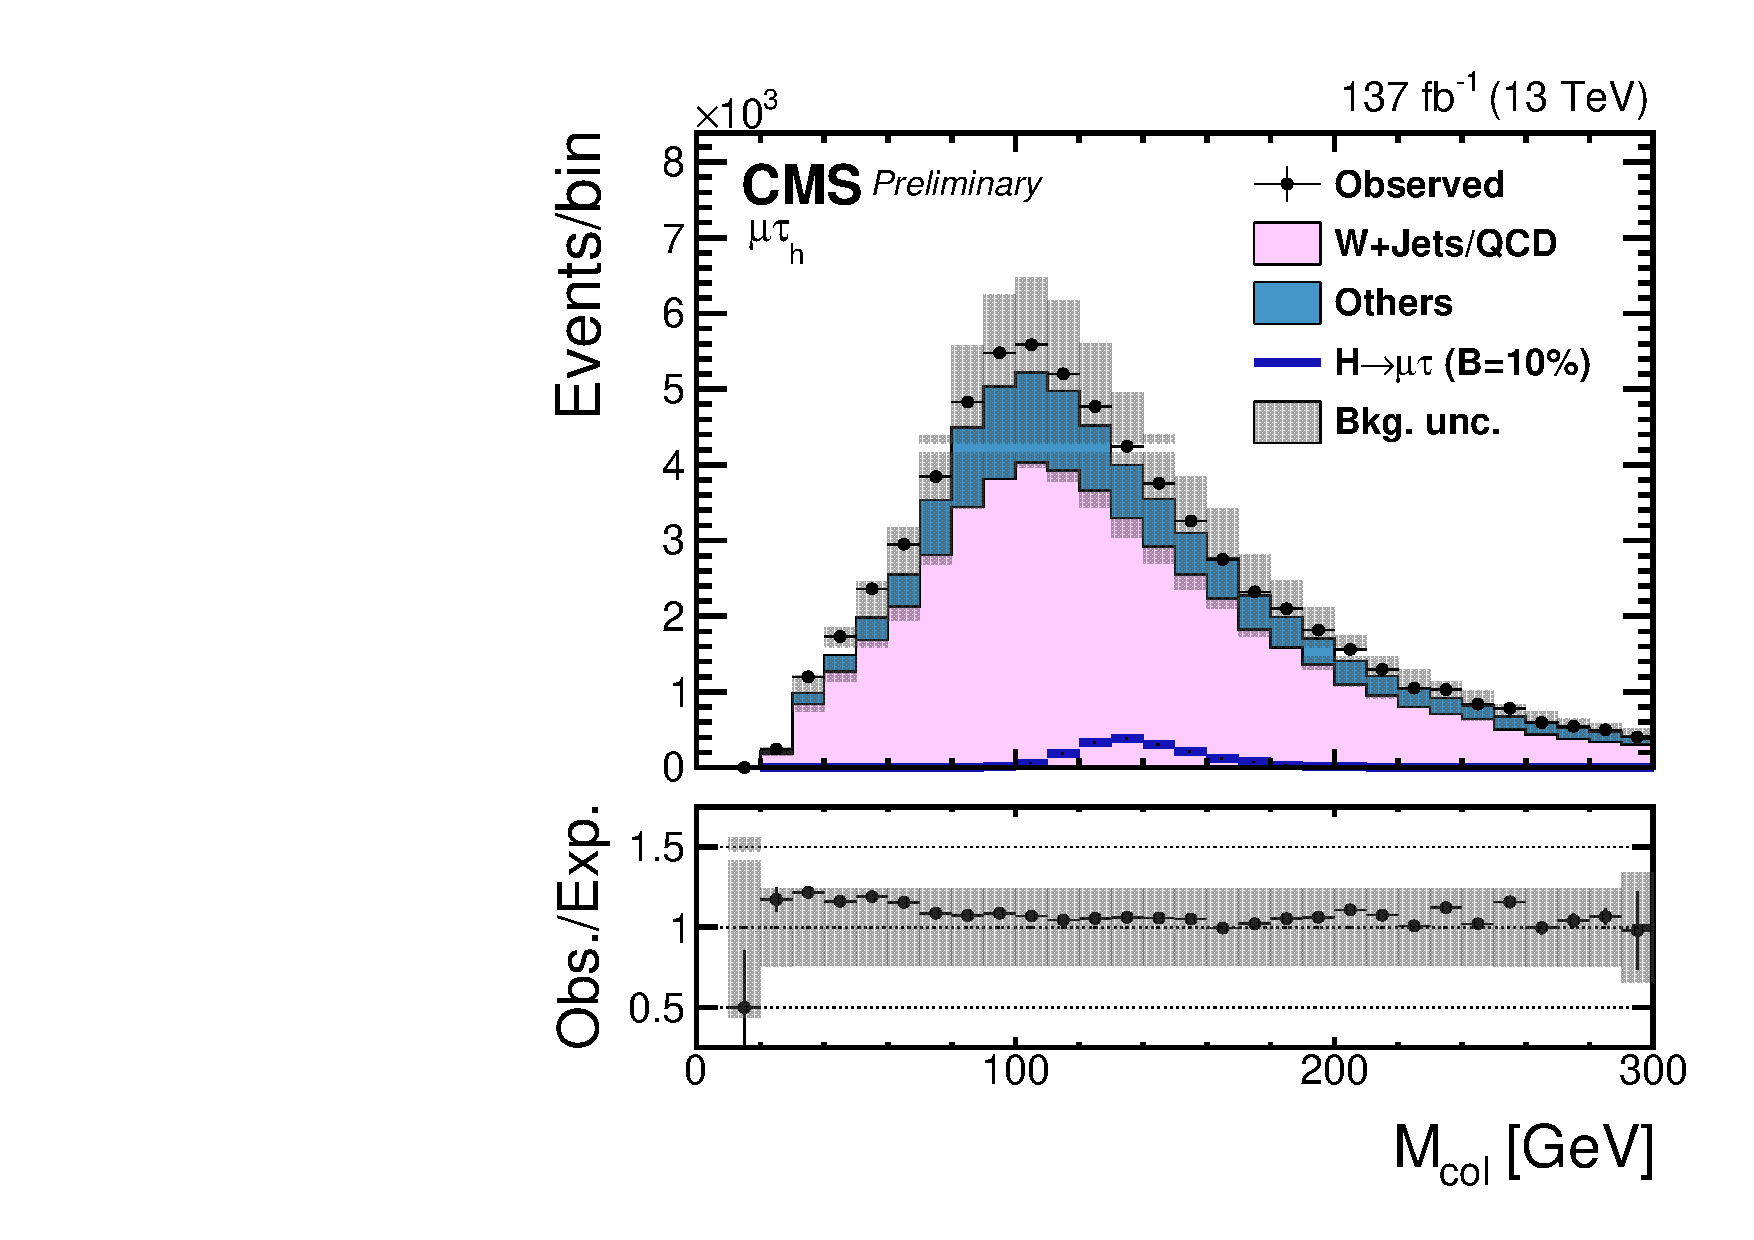
\includegraphics[width=0.45\textwidth]{plots/chapter7/Fake/mutau/WOS.pdf}
  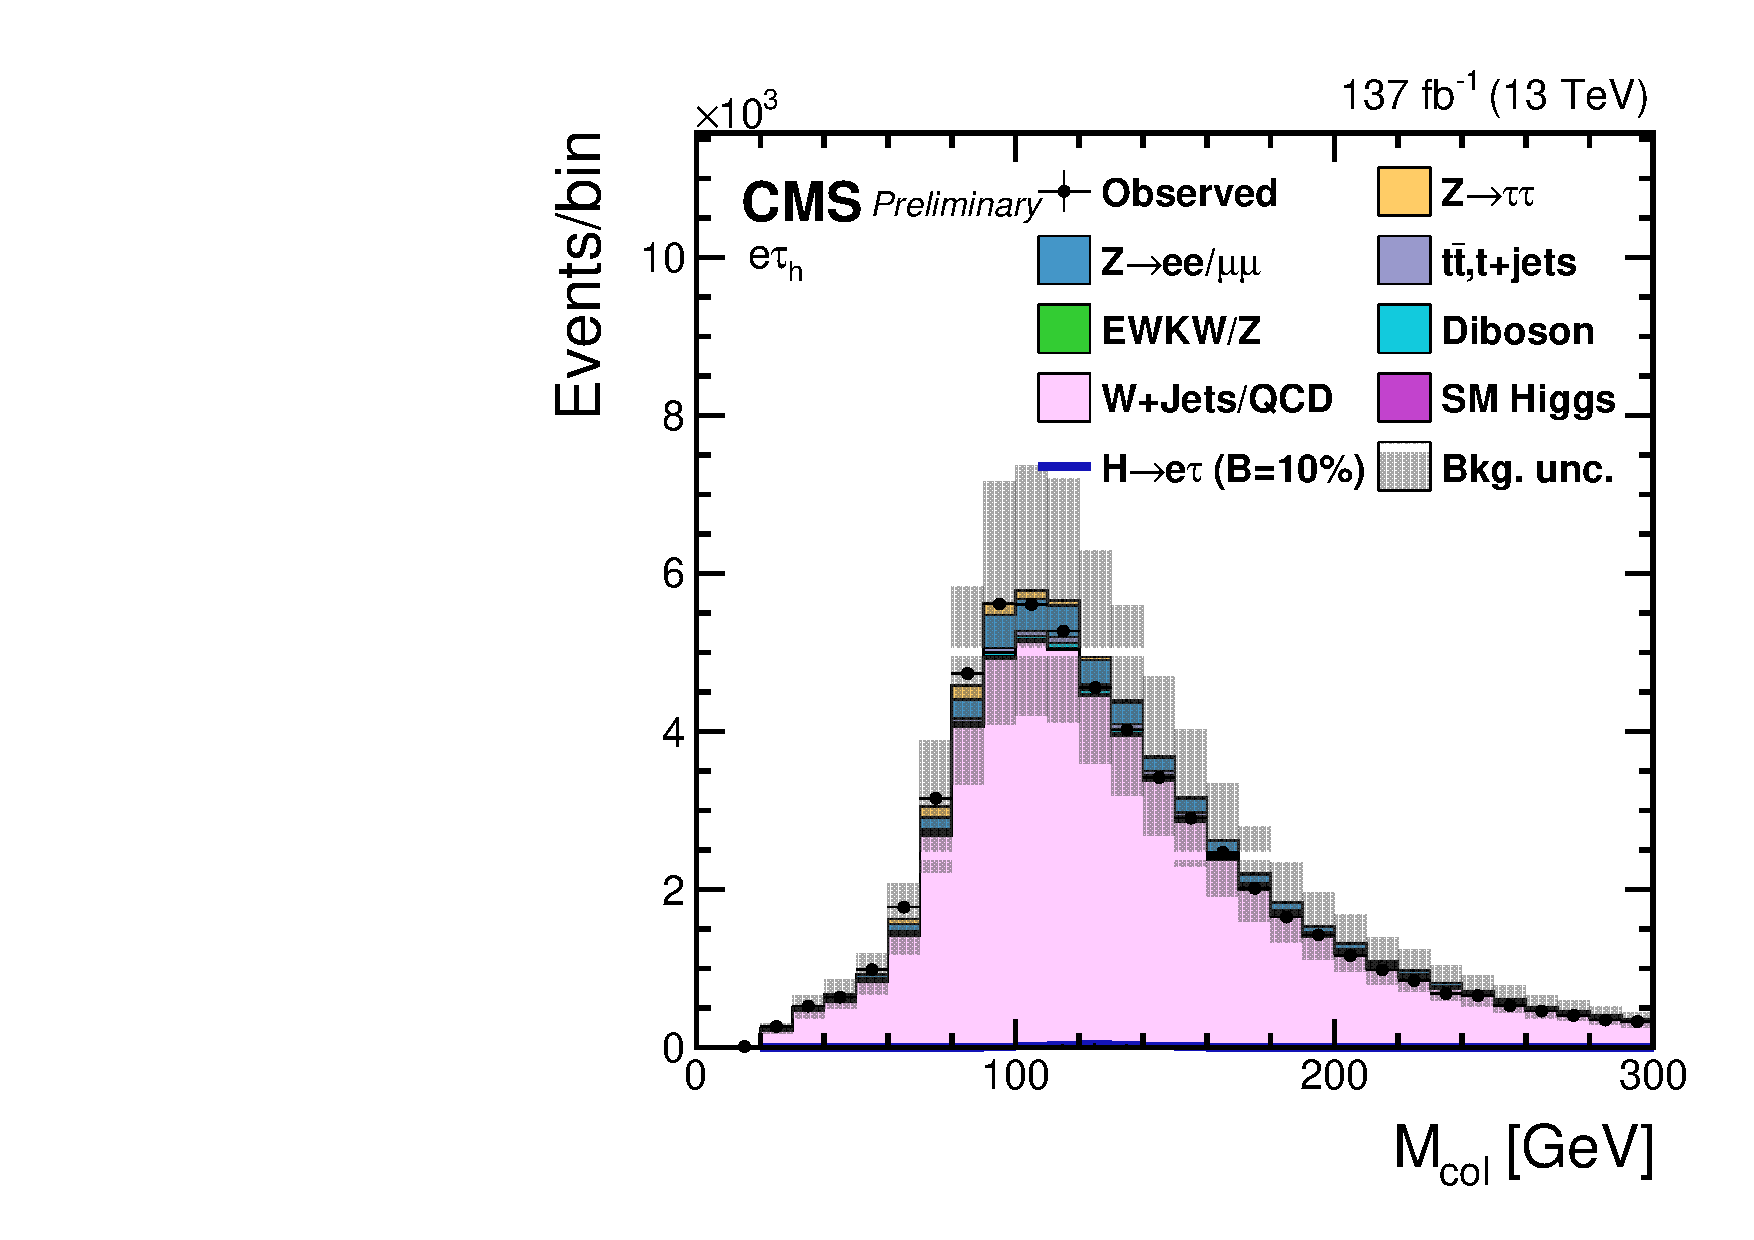
\includegraphics[width=0.45\textwidth]{plots/chapter7/Fake/etau/SS.pdf}
  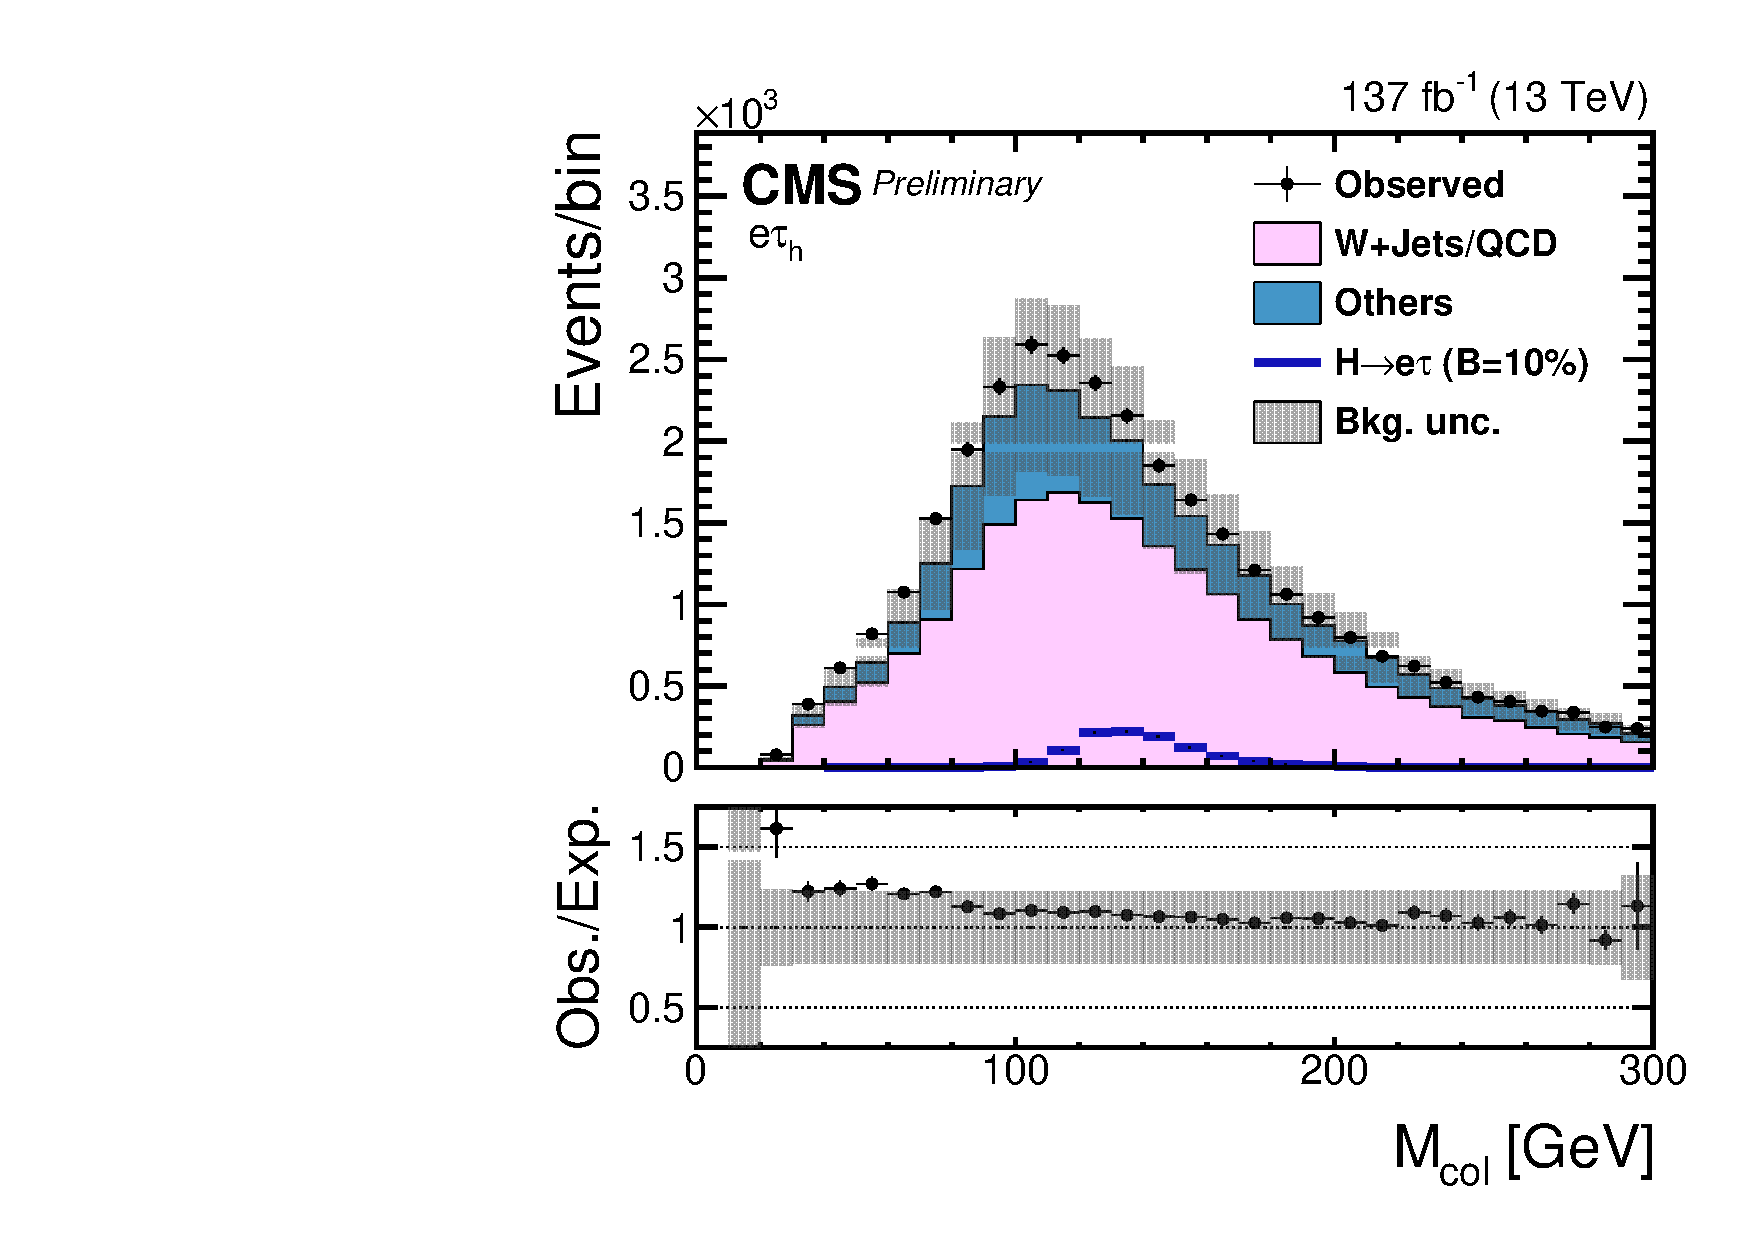
\includegraphics[width=0.45\textwidth]{plots/chapter7/Fake/etau/WOS.pdf}
  \caption{Distributions of \mcol discriminator in the same sign (left) and \PW boson enriched (right) control regions for the \muhad (top) and \ehad (bottom) channels.}
  \label{fig:fake_control}
\end{figure}

\begin{figure}[htbp!]
  \centering
  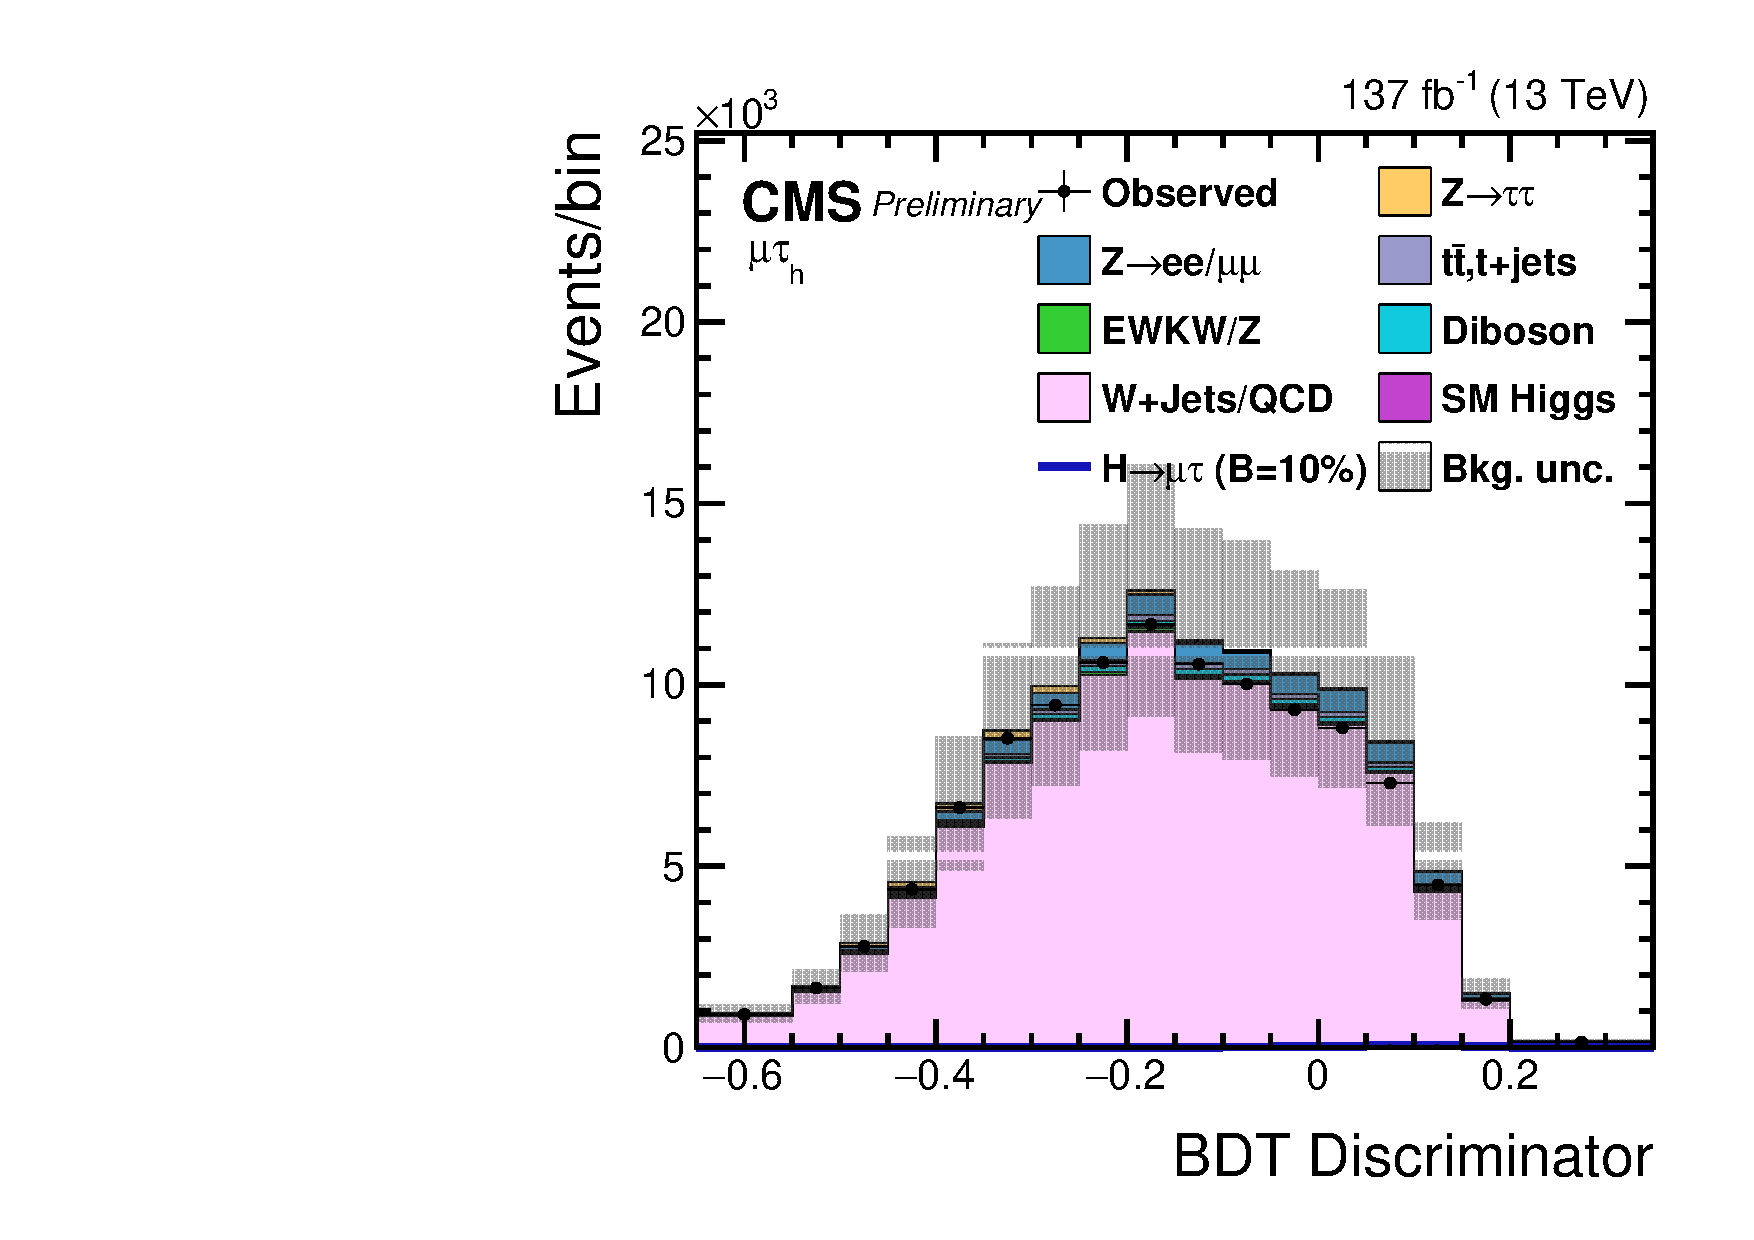
\includegraphics[width=0.45\textwidth]{plots/chapter7/Fake/mutau/SSBDT.pdf}
  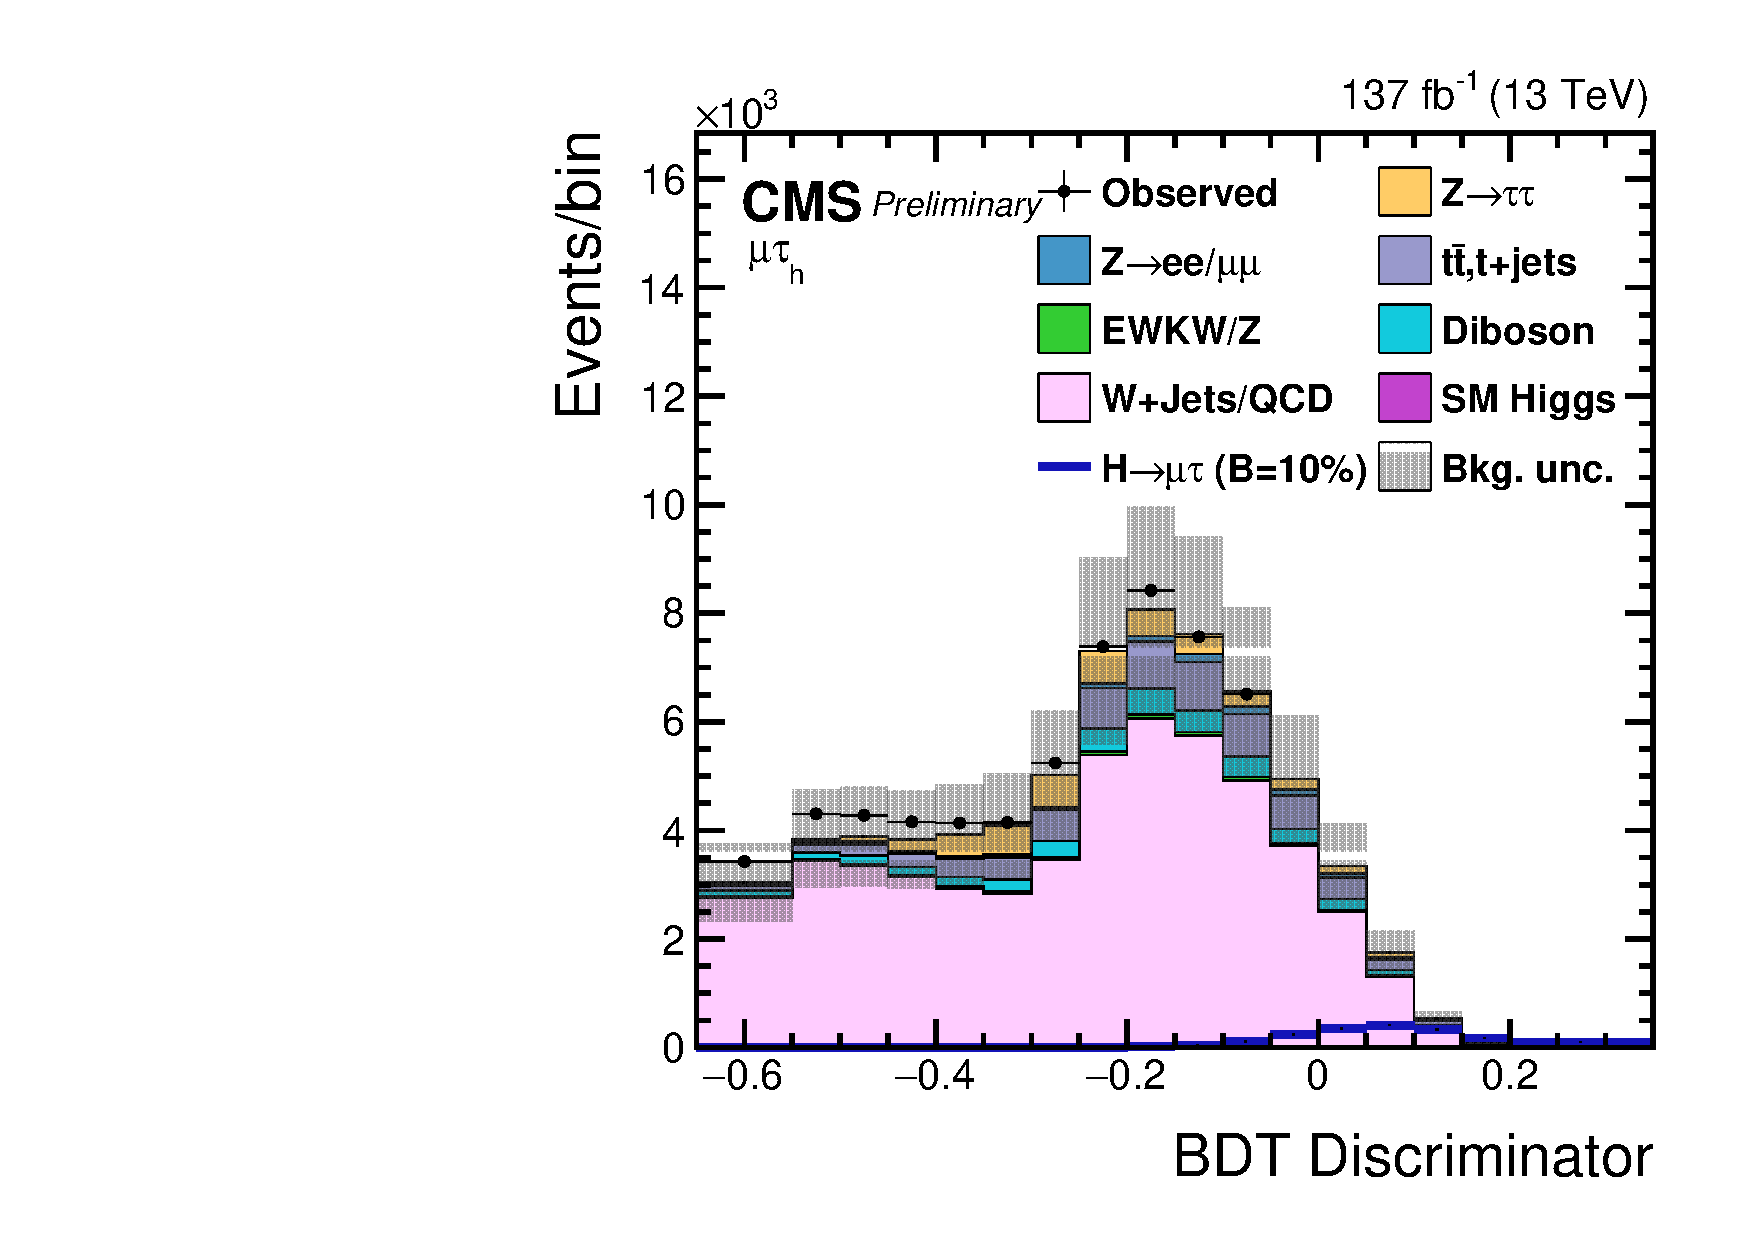
\includegraphics[width=0.45\textwidth]{plots/chapter7/Fake/mutau/WOSBDT.pdf}
  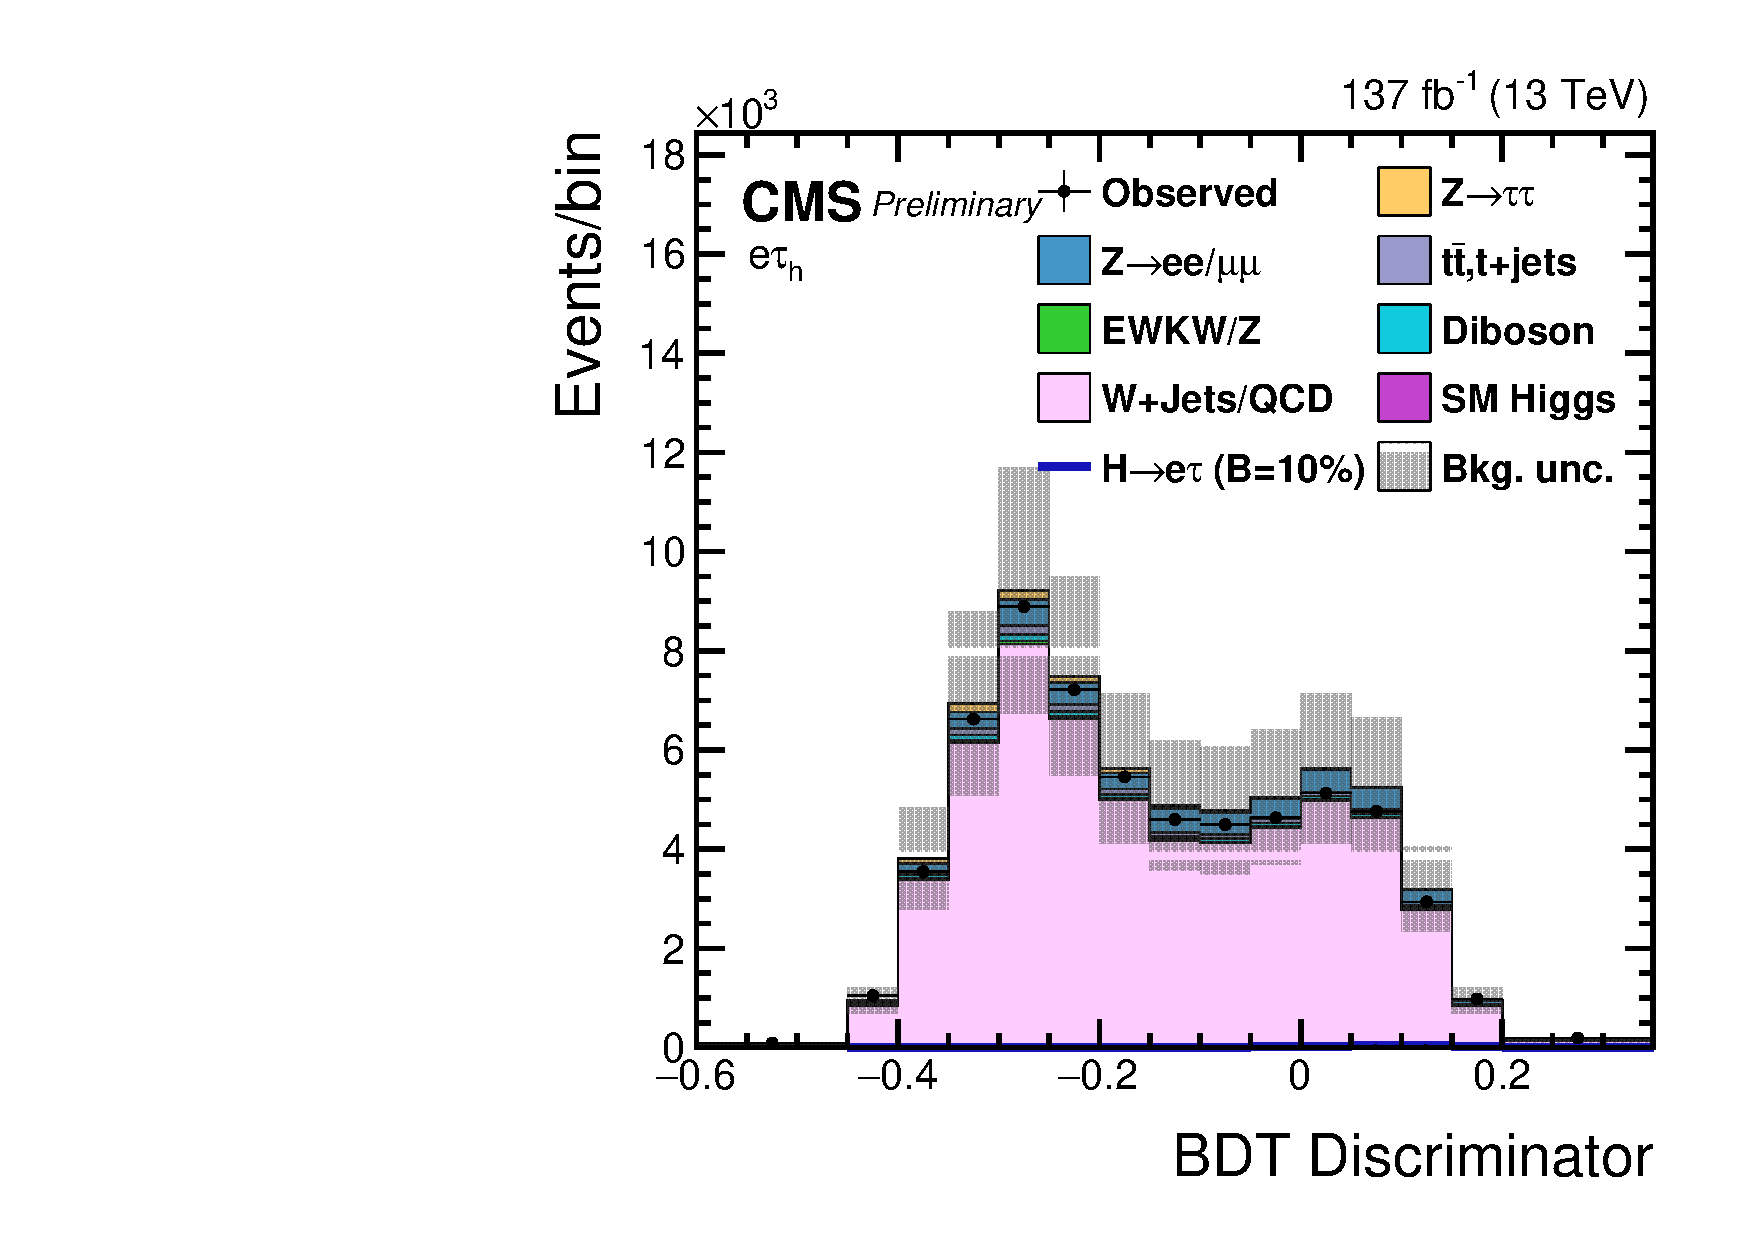
\includegraphics[width=0.45\textwidth]{plots/chapter7/Fake/etau/SSBDT.pdf}
  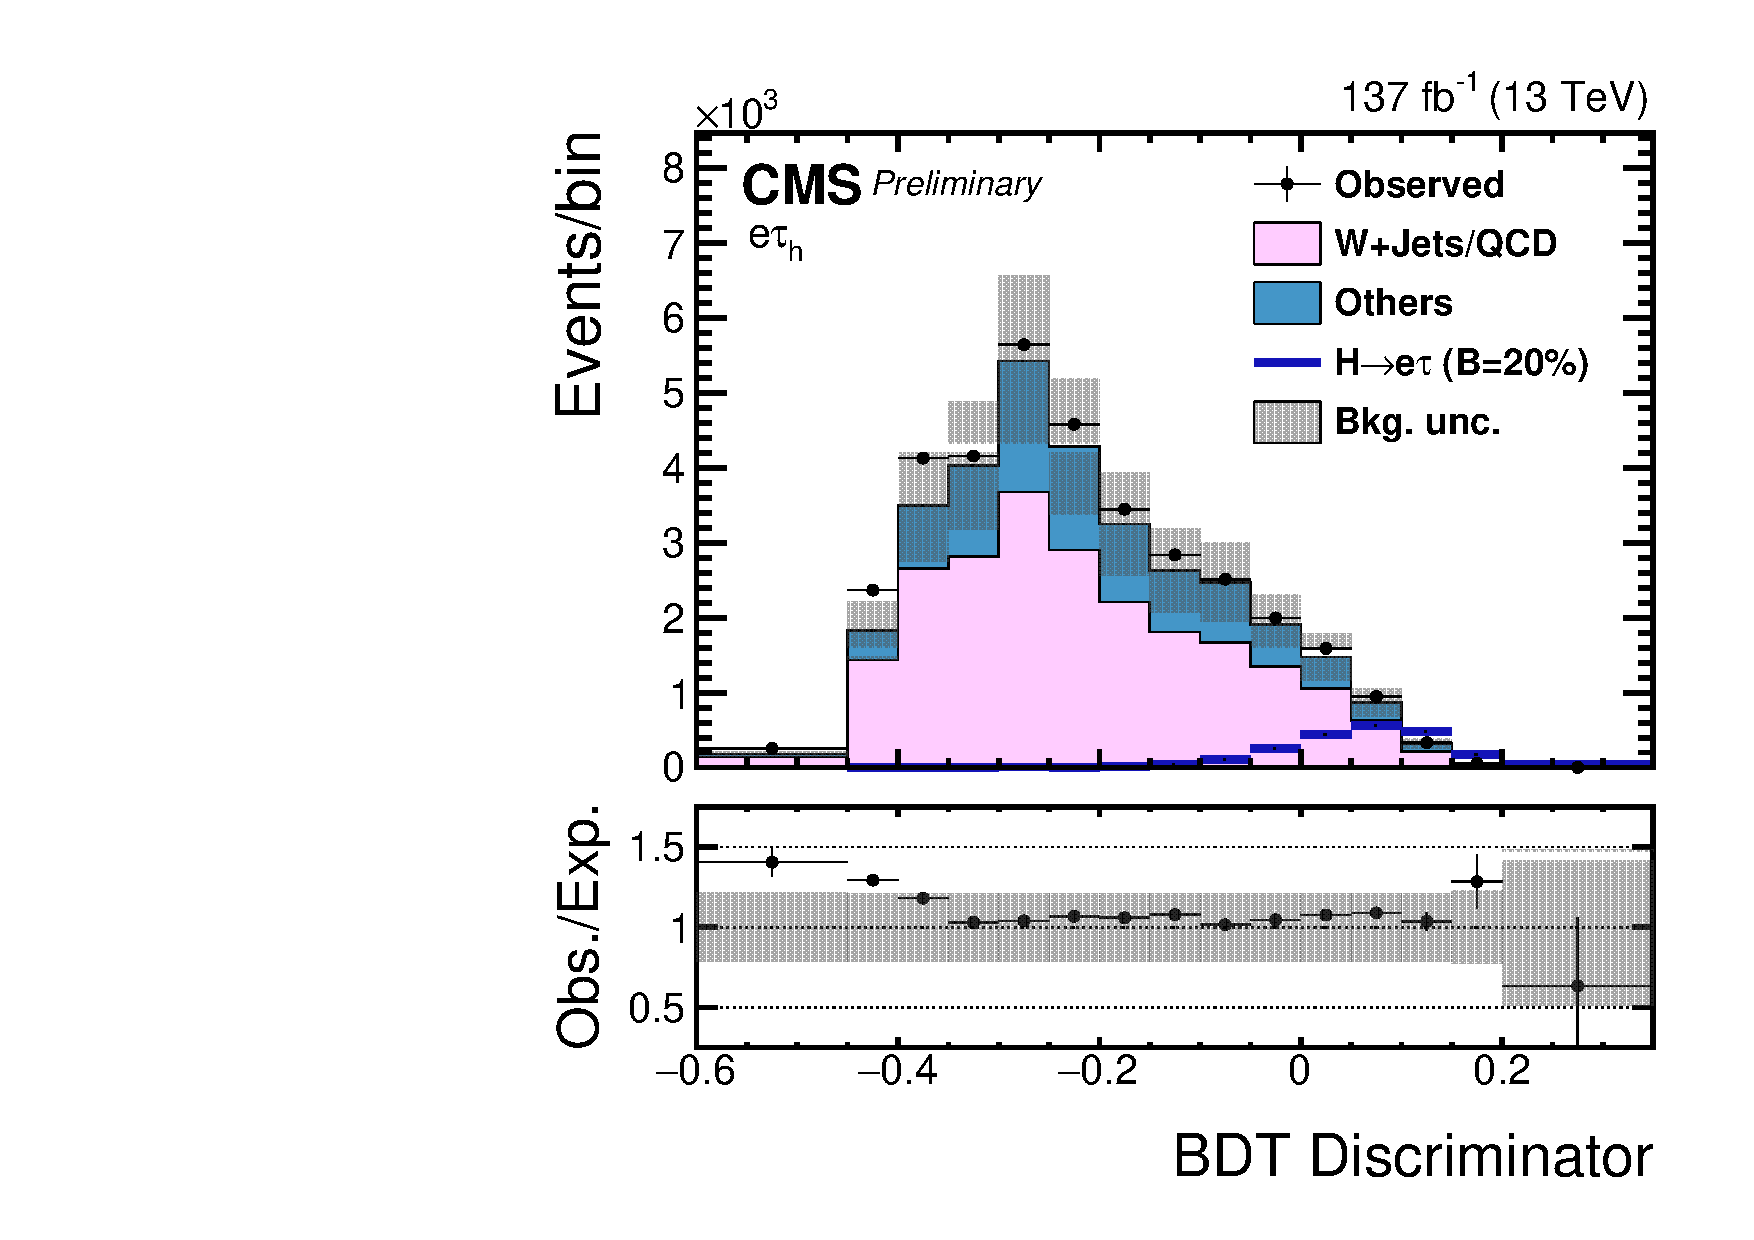
\includegraphics[width=0.45\textwidth]{plots/chapter7/Fake/etau/WOSBDT.pdf}
  \caption{Distributions of BDT discriminator in the same sign (left) and \PW boson enriched (right) control regions for the \muhad (top) and \ehad (bottom) channels.}
  \label{fig:fake_control_BDT}
\end{figure}

\subsection{Semi data-driven approach}
In the \emu and \mue channels, QCD multijet background is estimated from the data using events with an electron and a muon with the same electric charge. Contributions from other processes are estimated from simulation and subtracted from data. Extrapolation factors from the control region with the same electric charge for both the leptons to the signal region with an opposite electric charge for both the leptons are measured in data as a function of the jet multiplicity and the \dr separation between the electron and the muon. The extrapolation factors measured can be seen in Figure~\ref{fig:osss}.

\begin{figure}[htbp]
  \centering
  \subfigure[]{
    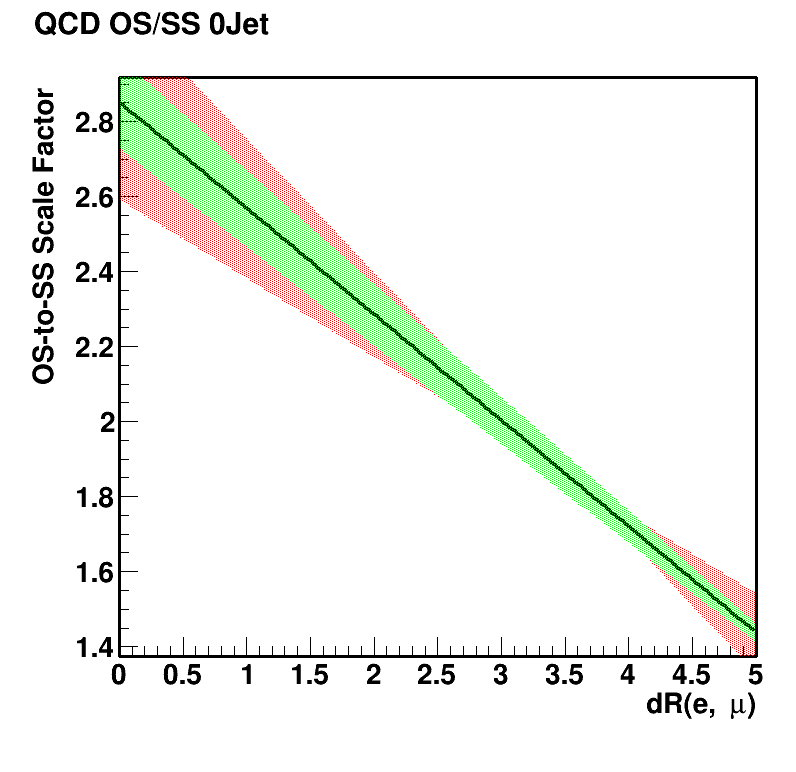
\includegraphics[width=0.3\textwidth]{plots/chapter7/QCD/2016/0Jet.png}
    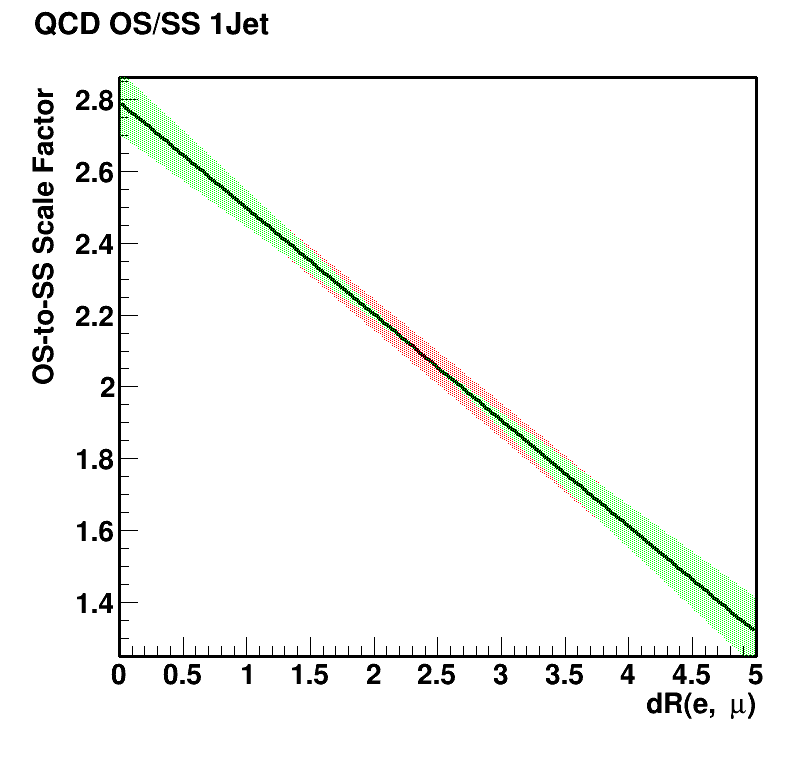
\includegraphics[width=0.3\textwidth]{plots/chapter7/QCD/2016/1Jet.png}
    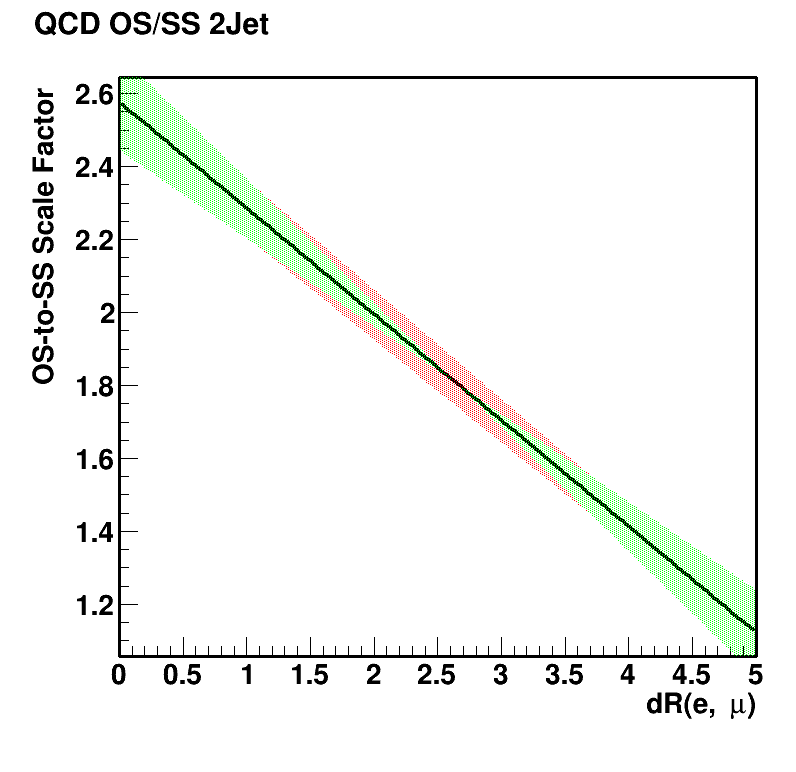
\includegraphics[width=0.3\textwidth]{plots/chapter7/QCD/2016/2Jet.png}
  }
  \subfigure[]{
    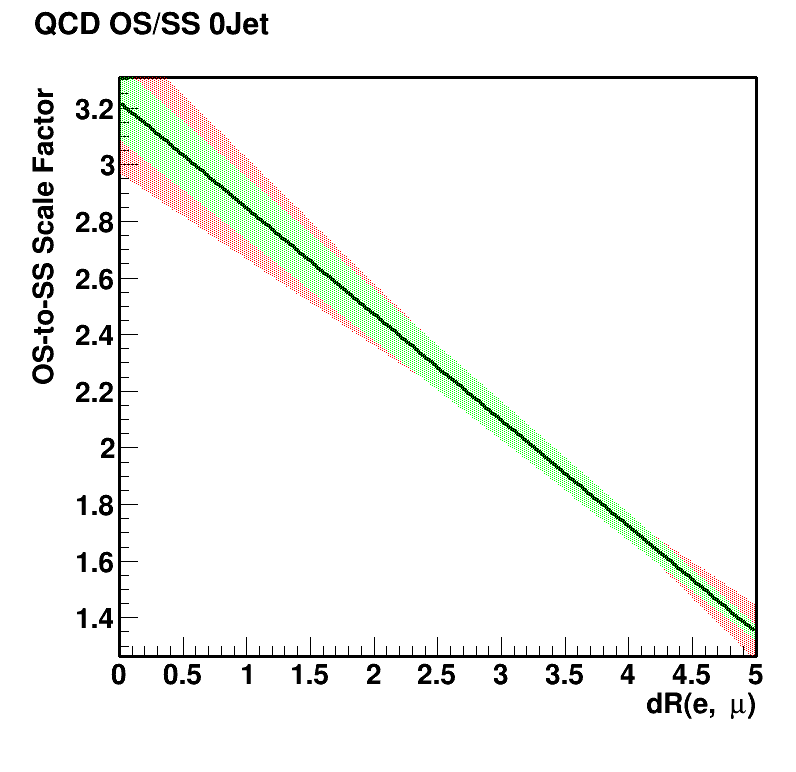
\includegraphics[width=0.3\textwidth]{plots/chapter7/QCD/2017/0Jet.png}
    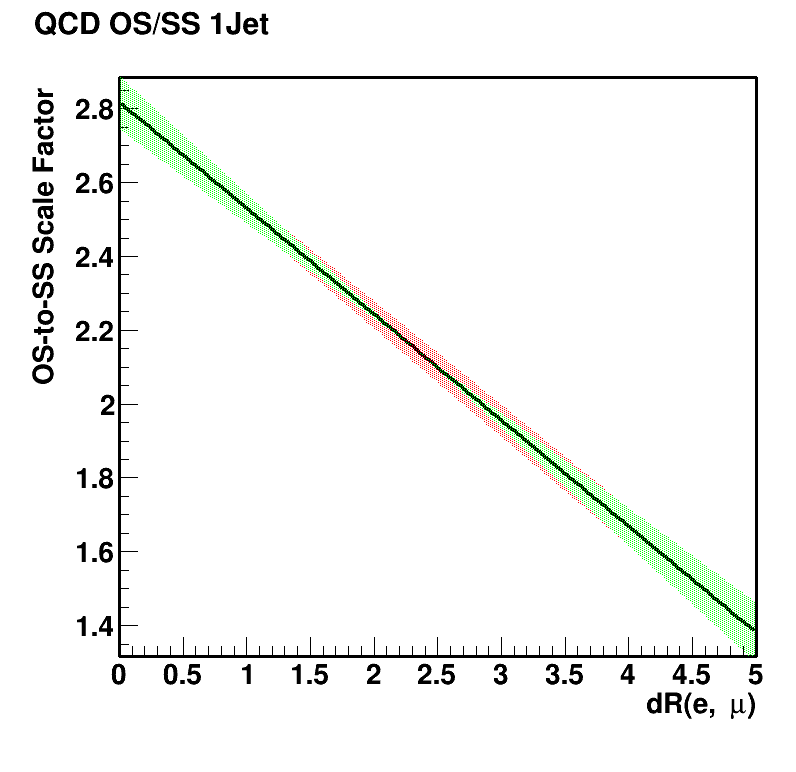
\includegraphics[width=0.3\textwidth]{plots/chapter7/QCD/2017/1Jet.png}
    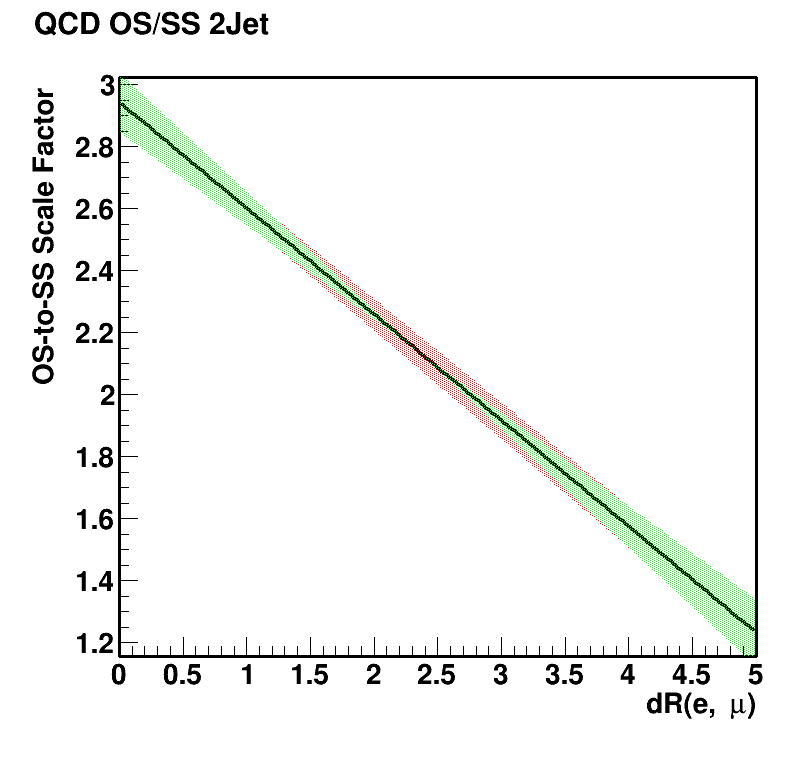
\includegraphics[width=0.3\textwidth]{plots/chapter7/QCD/2017/2Jet.png}
  }
  \subfigure[]{
    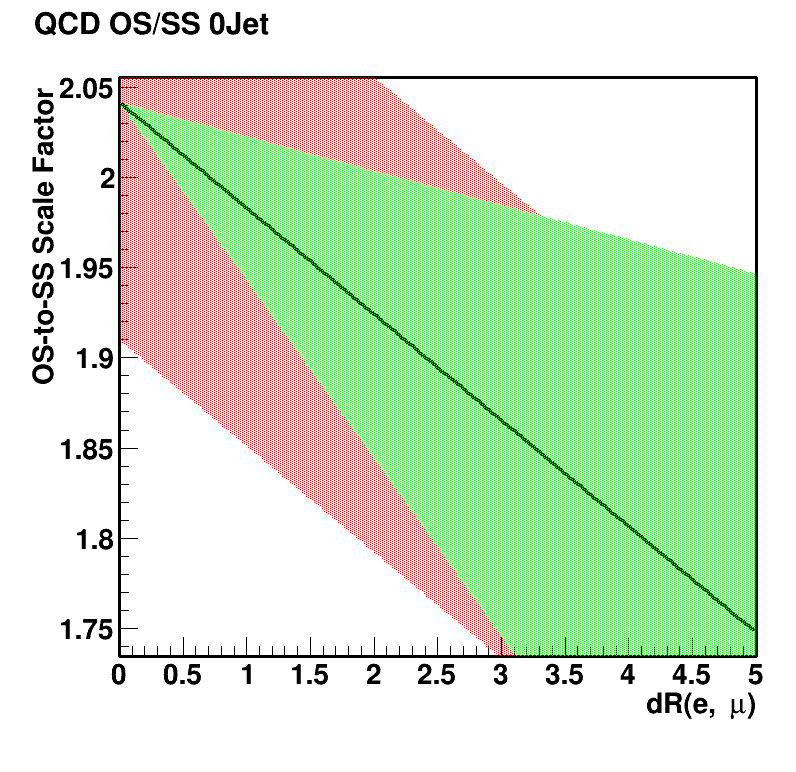
\includegraphics[width=0.3\textwidth]{plots/chapter7/QCD/2018/0Jet.png}
    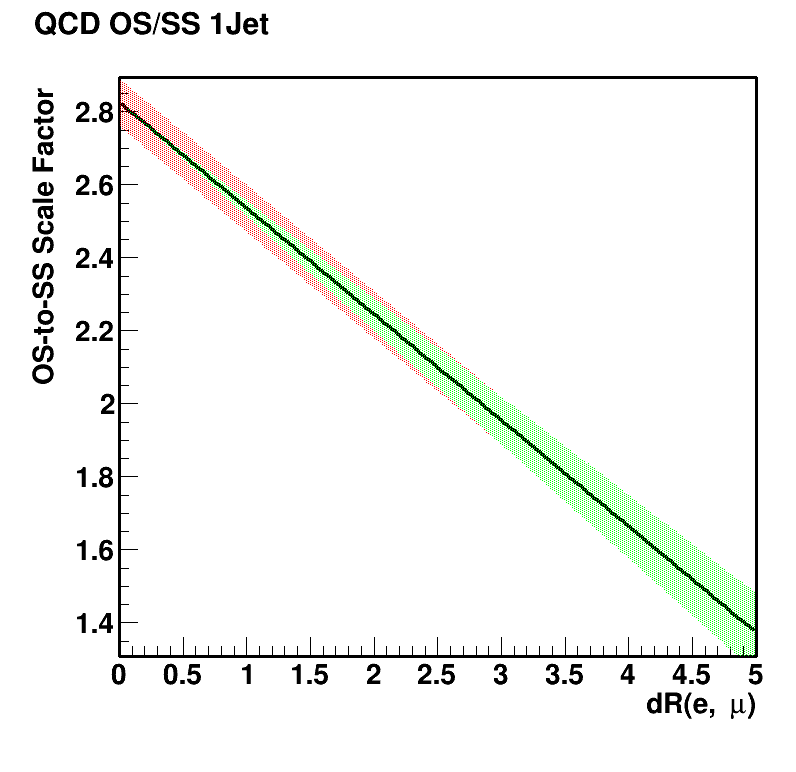
\includegraphics[width=0.3\textwidth]{plots/chapter7/QCD/2018/1Jet.png}
    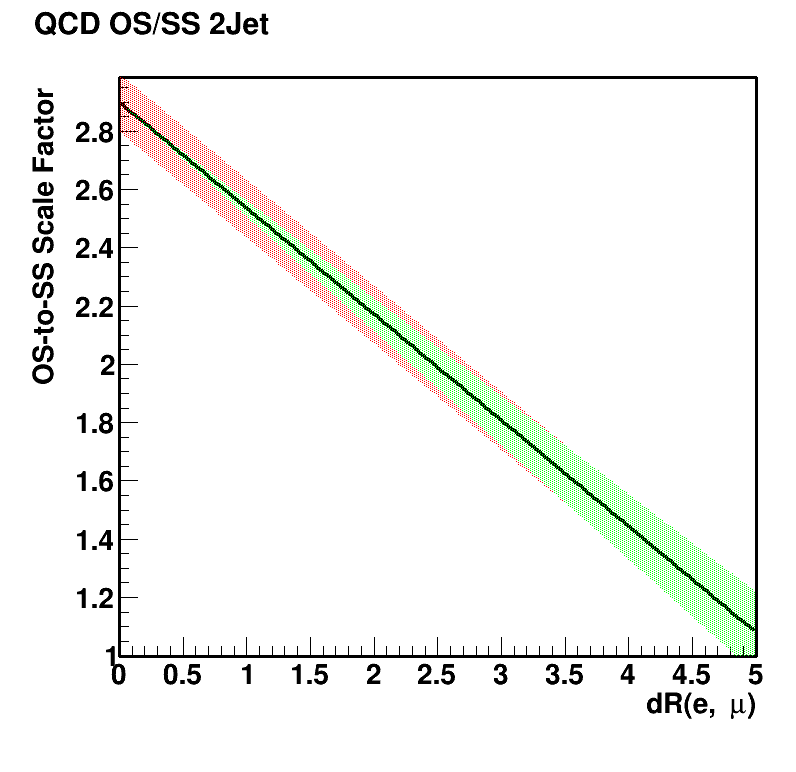
\includegraphics[width=0.3\textwidth]{plots/chapter7/QCD/2018/2Jet.png}
  }
  \caption{The extrapolation factors in events with 0 jets (left), 1 jet (center), and 2 jets (right) for 2016 (a), 2017 (b), 2018 (c). The line is the best fit, and the shaded region corresponds to the shape uncertainties.}
  \label{fig:osss}
\end{figure}

The extrapolation factors are estimated using events with an anti-isolated muon and an isolated electron. The contribution from \bbarb events to the QCD multijet background gives rise to the \dr dependency and is parameterized with a linear function. The extrapolation factors are higher for events with low \dr separation between the electron and the muon, decreasing as the \dr separation increases. The extrapolation factors also depend on the electron and muon \pt. This \pt dependence comes from the leptons arising from the semi-leptonic c quark decay. These leptons tend to be softer in \pt and less isolated resulting in a reduction in the number of such events passing the \pt and isolation requirements. Corrections of the extrapolation factors dependent on lepton \pt along with the correction to account for the mismodeling introduced by anti-isolating the muon to measure them can be seen in Figure~\ref{fig:osss_corr}.

\begin{figure}[htbp]
  \centering
  \subfigure[]{
    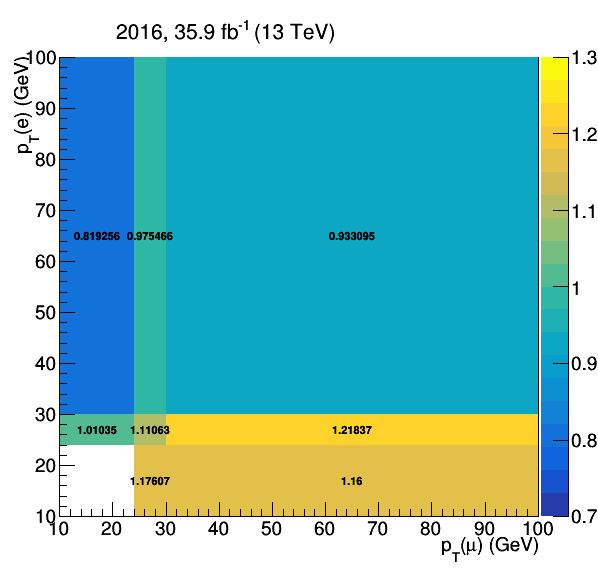
\includegraphics[width=0.3\textwidth]{plots/chapter7/QCD/2016/pt.png}
    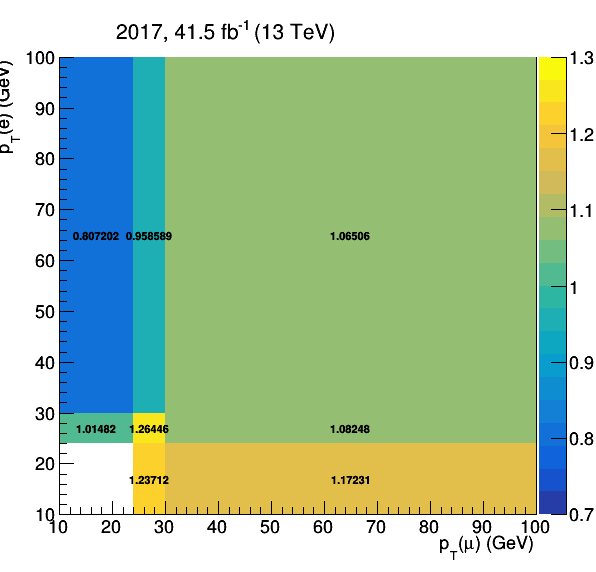
\includegraphics[width=0.3\textwidth]{plots/chapter7/QCD/2017/pt.png}
    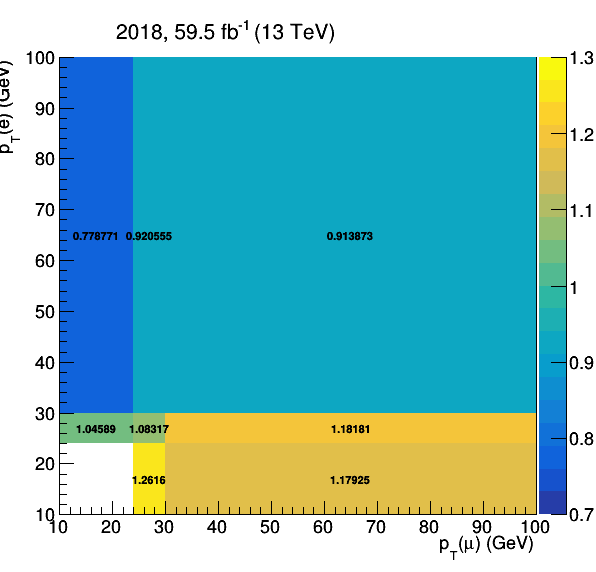
\includegraphics[width=0.3\textwidth]{plots/chapter7/QCD/2018/pt.png}
  }
  \subfigure[]{
    \includegraphics[width=0.3\textwidth]{plots/chapter7/QCD/2016/iso.png}
    \includegraphics[width=0.3\textwidth]{plots/chapter7/QCD/2017/iso.png}
    \includegraphics[width=0.3\textwidth]{plots/chapter7/QCD/2018/iso.png}
  }
  \caption{(a) Corrections of the QCD OS/SS extrapolation factors determined in the region with an anti-isolated muon as a function of the \pt of the electron and the muon, using data collected in 2016, 2017, and 2018. (b) Correction of the QCD OS/SS extrapolation factors to account for the mismodeling introduced by anti-isolating the muon to measure the SFs, using data collected in 2016, 2017, and 2018.}
  \label{fig:osss_corr}
\end{figure}

As the extrapolation factors are measured in a control region where the muon is anti-isolated, an additional correction is applied to cover a potential mismodeling. This correction is calculated by measuring the extrapolation factors in two different control regions. The first control region has events where the muon is isolated, and the electron is anti-isolated. The second control region has events where both the electron and the muon are anti-isolated. The ratio of the extrapolation factors measured in these two control regions is taken as the correction for accounting for the potential mismodeling induced by anti-isolating the muon. Figure~\ref{fig:qcd_control} shows the comparison of data with estimated background in the muon anti-isolated control regions for the \mue channel.

\begin{figure}[htbp!]
  \centering
  \includegraphics[width=0.45\textwidth]{plots/chapter7/Fake/mue/QCD.pdf}
  \caption{Distribution of \mcol discriminator in the muon anti-isolated control regions for the \mue channel.}
  \label{fig:qcd_control}
\end{figure}

\section{Monte Carlo simulations}
All the other backgrounds are estimated using MC simulation. In the leptonic channels, the \ttbar process has a dominant contribution. This background is validated in a dedicated control region defined by requiring at least one b jet tagged by the DeepCSV algorithm in the event. Figure~\ref{fig:tt_control} shows the background validation in this control region for the \mue and \emu channels.

The SM Higgs boson production forms a small but non-negligible background. The contributions come mainly from \Htt and \HWW decays. The contribution from \HWW peaks at lower values than the signal in the distribution of the BDT discriminator due to the presence of additional neutrinos in the decay.

\begin{figure}[htbp!]
  \centering
  \includegraphics[width=0.45\textwidth]{plots/chapter7/Fake/mue/TT.pdf}
  \includegraphics[width=0.45\textwidth]{plots/chapter7/Fake/emu/TT.pdf}
  \includegraphics[width=0.45\textwidth]{plots/chapter7/Fake/mue/TTBDT.pdf}
  \includegraphics[width=0.45\textwidth]{plots/chapter7/Fake/emu/TTBDT.pdf}
  \caption{Distributions of \mcol (BDT) discriminator in \ttbar enriched control region for \mue and \emu channel.}
  \label{fig:tt_control}
\end{figure}
